% Options for packages loaded elsewhere
\PassOptionsToPackage{unicode}{hyperref}
\PassOptionsToPackage{hyphens}{url}
%
\documentclass[
  spanish,
]{article}
\usepackage{lmodern}
\usepackage{amssymb,amsmath}
\usepackage{ifxetex,ifluatex}
\ifnum 0\ifxetex 1\fi\ifluatex 1\fi=0 % if pdftex
  \usepackage[T1]{fontenc}
  \usepackage[utf8]{inputenc}
  \usepackage{textcomp} % provide euro and other symbols
\else % if luatex or xetex
  \usepackage{unicode-math}
  \defaultfontfeatures{Scale=MatchLowercase}
  \defaultfontfeatures[\rmfamily]{Ligatures=TeX,Scale=1}
\fi
% Use upquote if available, for straight quotes in verbatim environments
\IfFileExists{upquote.sty}{\usepackage{upquote}}{}
\IfFileExists{microtype.sty}{% use microtype if available
  \usepackage[]{microtype}
  \UseMicrotypeSet[protrusion]{basicmath} % disable protrusion for tt fonts
}{}
\makeatletter
\@ifundefined{KOMAClassName}{% if non-KOMA class
  \IfFileExists{parskip.sty}{%
    \usepackage{parskip}
  }{% else
    \setlength{\parindent}{0pt}
    \setlength{\parskip}{6pt plus 2pt minus 1pt}}
}{% if KOMA class
  \KOMAoptions{parskip=half}}
\makeatother
\usepackage{xcolor}
\IfFileExists{xurl.sty}{\usepackage{xurl}}{} % add URL line breaks if available
\IfFileExists{bookmark.sty}{\usepackage{bookmark}}{\usepackage{hyperref}}
\hypersetup{
  pdfauthor={Emilio Alarcón Martín},
  hidelinks,
  pdfcreator={LaTeX via pandoc}}
\urlstyle{same} % disable monospaced font for URLs
\usepackage[margin=1in]{geometry}
\usepackage{color}
\usepackage{fancyvrb}
\newcommand{\VerbBar}{|}
\newcommand{\VERB}{\Verb[commandchars=\\\{\}]}
\DefineVerbatimEnvironment{Highlighting}{Verbatim}{commandchars=\\\{\}}
% Add ',fontsize=\small' for more characters per line
\usepackage{framed}
\definecolor{shadecolor}{RGB}{248,248,248}
\newenvironment{Shaded}{\begin{snugshade}}{\end{snugshade}}
\newcommand{\AlertTok}[1]{\textcolor[rgb]{0.94,0.16,0.16}{#1}}
\newcommand{\AnnotationTok}[1]{\textcolor[rgb]{0.56,0.35,0.01}{\textbf{\textit{#1}}}}
\newcommand{\AttributeTok}[1]{\textcolor[rgb]{0.77,0.63,0.00}{#1}}
\newcommand{\BaseNTok}[1]{\textcolor[rgb]{0.00,0.00,0.81}{#1}}
\newcommand{\BuiltInTok}[1]{#1}
\newcommand{\CharTok}[1]{\textcolor[rgb]{0.31,0.60,0.02}{#1}}
\newcommand{\CommentTok}[1]{\textcolor[rgb]{0.56,0.35,0.01}{\textit{#1}}}
\newcommand{\CommentVarTok}[1]{\textcolor[rgb]{0.56,0.35,0.01}{\textbf{\textit{#1}}}}
\newcommand{\ConstantTok}[1]{\textcolor[rgb]{0.00,0.00,0.00}{#1}}
\newcommand{\ControlFlowTok}[1]{\textcolor[rgb]{0.13,0.29,0.53}{\textbf{#1}}}
\newcommand{\DataTypeTok}[1]{\textcolor[rgb]{0.13,0.29,0.53}{#1}}
\newcommand{\DecValTok}[1]{\textcolor[rgb]{0.00,0.00,0.81}{#1}}
\newcommand{\DocumentationTok}[1]{\textcolor[rgb]{0.56,0.35,0.01}{\textbf{\textit{#1}}}}
\newcommand{\ErrorTok}[1]{\textcolor[rgb]{0.64,0.00,0.00}{\textbf{#1}}}
\newcommand{\ExtensionTok}[1]{#1}
\newcommand{\FloatTok}[1]{\textcolor[rgb]{0.00,0.00,0.81}{#1}}
\newcommand{\FunctionTok}[1]{\textcolor[rgb]{0.00,0.00,0.00}{#1}}
\newcommand{\ImportTok}[1]{#1}
\newcommand{\InformationTok}[1]{\textcolor[rgb]{0.56,0.35,0.01}{\textbf{\textit{#1}}}}
\newcommand{\KeywordTok}[1]{\textcolor[rgb]{0.13,0.29,0.53}{\textbf{#1}}}
\newcommand{\NormalTok}[1]{#1}
\newcommand{\OperatorTok}[1]{\textcolor[rgb]{0.81,0.36,0.00}{\textbf{#1}}}
\newcommand{\OtherTok}[1]{\textcolor[rgb]{0.56,0.35,0.01}{#1}}
\newcommand{\PreprocessorTok}[1]{\textcolor[rgb]{0.56,0.35,0.01}{\textit{#1}}}
\newcommand{\RegionMarkerTok}[1]{#1}
\newcommand{\SpecialCharTok}[1]{\textcolor[rgb]{0.00,0.00,0.00}{#1}}
\newcommand{\SpecialStringTok}[1]{\textcolor[rgb]{0.31,0.60,0.02}{#1}}
\newcommand{\StringTok}[1]{\textcolor[rgb]{0.31,0.60,0.02}{#1}}
\newcommand{\VariableTok}[1]{\textcolor[rgb]{0.00,0.00,0.00}{#1}}
\newcommand{\VerbatimStringTok}[1]{\textcolor[rgb]{0.31,0.60,0.02}{#1}}
\newcommand{\WarningTok}[1]{\textcolor[rgb]{0.56,0.35,0.01}{\textbf{\textit{#1}}}}
\usepackage{graphicx,grffile}
\makeatletter
\def\maxwidth{\ifdim\Gin@nat@width>\linewidth\linewidth\else\Gin@nat@width\fi}
\def\maxheight{\ifdim\Gin@nat@height>\textheight\textheight\else\Gin@nat@height\fi}
\makeatother
% Scale images if necessary, so that they will not overflow the page
% margins by default, and it is still possible to overwrite the defaults
% using explicit options in \includegraphics[width, height, ...]{}
\setkeys{Gin}{width=\maxwidth,height=\maxheight,keepaspectratio}
% Set default figure placement to htbp
\makeatletter
\def\fps@figure{htbp}
\makeatother
\setlength{\emergencystretch}{3em} % prevent overfull lines
\providecommand{\tightlist}{%
  \setlength{\itemsep}{0pt}\setlength{\parskip}{0pt}}
\setcounter{secnumdepth}{-\maxdimen} % remove section numbering
\ifxetex
  % Load polyglossia as late as possible: uses bidi with RTL langages (e.g. Hebrew, Arabic)
  \usepackage{polyglossia}
  \setmainlanguage[]{spanish}
\else
  \usepackage[shorthands=off,main=spanish]{babel}
\fi

\title{Análisis de datos de Microarrays\\
PEC1 - Análisis de Datos ómicos}
\author{Emilio Alarcón Martín}
\date{3 de mayo, 2020}

\begin{document}
\maketitle

{
\setcounter{tocdepth}{4}
\tableofcontents
}
\hypertarget{introducciuxf3n}{%
\section{Introducción}\label{introducciuxf3n}}

\hypertarget{objetivo}{%
\subsection{Objetivo}\label{objetivo}}

El objetivo de este trabajo es realizar un análisis de datos de
microarrays del set de datos seleccionado, GDS2300. Consta de 6 muestras
de ovocitos de ratón. Compararemos la expresión génica de 3 ovocitos en
estadio de metafase II con 3 ovocitos en estadio de vesícula germinal.

\hypertarget{abstract}{%
\subsection{Abstract}\label{abstract}}

En este artículo se buscó identificar y caracterizar las transcripciones
que están degradadas frente a las que están estables durante la
transición de la vesícula germinal (VG) transcriptivamente silenciosa a
la metafase II (MII) mediante un enfoque de microarrays. Se utilizó un
sistema de amplificación de la transcripción de los ovocitos utilizando
cebado interno y de 3'-poly(A) para minimizar el impacto de las
variaciones complejas en la poliadenilación de la transcripción que
prevalecen durante esta transición. Las transcripciones fueron
identificadas y cuantificadas usando el genoma del ratón Affymetrix 430
v2.0 GeneChip.

\href{https://www.ncbi.nlm.nih.gov/pubmed/17022963}{\emph{Su, Y. Q.,
Sugiura, K., Woo, Y., Wigglesworth, K., Kamdar, S., Affourtit, J., \&
Eppig, J. J. (2007). Selective degradation of transcripts during meiotic
maturation of mouse oocytes. Developmental biology, 302(1), 104-117.}}

\hypertarget{puesta-a-punto-de-rstudio}{%
\subsection{Puesta a punto de Rstudio}\label{puesta-a-punto-de-rstudio}}

Se plantea aquí la instalación de los paquetes y su activación en
Rstudio para su uso en esta actividad. Podrían no coincidir las
versiones de los paquetes con las realizadas posteriormente.

\begin{Shaded}
\begin{Highlighting}[]
\OperatorTok{>}\StringTok{ }\ControlFlowTok{if}\NormalTok{ (}\OperatorTok{!}\KeywordTok{requireNamespace}\NormalTok{(}\StringTok{"BiocManager"}\NormalTok{, }\DataTypeTok{quietly =} \OtherTok{TRUE}\NormalTok{))}
\OperatorTok{+}\StringTok{     }\KeywordTok{install.packages}\NormalTok{(}\StringTok{"BiocManager"}\NormalTok{)}
\OperatorTok{>}\StringTok{ }\NormalTok{BiocManager}\OperatorTok{::}\KeywordTok{install}\NormalTok{()}
\OperatorTok{>}\StringTok{ }
\ErrorTok{>}\StringTok{ }
\ErrorTok{>}\StringTok{ }\NormalTok{libraries <-}\StringTok{ }\KeywordTok{c}\NormalTok{(}\StringTok{"affy"}\NormalTok{,}
\OperatorTok{+}\StringTok{                "annaffy"}\NormalTok{,}
\OperatorTok{+}\StringTok{                "annotate"}\NormalTok{,}
\OperatorTok{+}\StringTok{                "affyPLM"}\NormalTok{,}
\OperatorTok{+}\StringTok{                "affyQCReport"}\NormalTok{,}
\OperatorTok{+}\StringTok{                "genefilter"}\NormalTok{,}
\OperatorTok{+}\StringTok{                "limma"}\NormalTok{,}
\OperatorTok{+}\StringTok{                "org.Mm.eg.db"}\NormalTok{,}
\OperatorTok{+}\StringTok{                "mouse4302.db"}\NormalTok{,}
\OperatorTok{+}\StringTok{                "DOSE"}\NormalTok{,}
\OperatorTok{+}\StringTok{                "clusterProfiler"}\NormalTok{,}
\OperatorTok{+}\StringTok{                "pathview"}\NormalTok{,}
\OperatorTok{+}\StringTok{                "Category"}\NormalTok{,}
\OperatorTok{+}\StringTok{                "GO.db"}\NormalTok{,}
\OperatorTok{+}\StringTok{                "GOstats"}\NormalTok{,}
\OperatorTok{+}\StringTok{                "gplots"}\NormalTok{)}
\OperatorTok{>}\StringTok{ }
\ErrorTok{>}\StringTok{ }
\ErrorTok{>}\StringTok{ }\NormalTok{check.libraries <-}\StringTok{ }\KeywordTok{is.element}\NormalTok{(libraries, }\KeywordTok{installed.packages}\NormalTok{()[, }\DecValTok{1}\NormalTok{])}\OperatorTok{==}\OtherTok{FALSE}
\OperatorTok{>}\StringTok{ }\NormalTok{libraries.to.install <-}\StringTok{ }\NormalTok{libraries[check.libraries]}
\OperatorTok{>}\StringTok{ }\ControlFlowTok{if}\NormalTok{ (}\KeywordTok{length}\NormalTok{(libraries.to.install}\OperatorTok{!=}\DecValTok{0}\NormalTok{)) \{}
\OperatorTok{+}\StringTok{ }\ControlFlowTok{if}\NormalTok{ (}\OperatorTok{!}\KeywordTok{requireNamespace}\NormalTok{(}\StringTok{"BiocManager"}\NormalTok{, }\DataTypeTok{quietly =} \OtherTok{TRUE}\NormalTok{))}
\OperatorTok{+}\StringTok{   }\KeywordTok{install.packages}\NormalTok{(}\StringTok{"BiocManager"}\NormalTok{)}
\OperatorTok{+}\StringTok{ }\NormalTok{BiocManager}\OperatorTok{::}\KeywordTok{install}\NormalTok{(libraries.to.install)}
\OperatorTok{+}\StringTok{ }\NormalTok{\}}
\OperatorTok{>}\StringTok{ }
\ErrorTok{>}\StringTok{ }\ControlFlowTok{for}\NormalTok{ (i }\ControlFlowTok{in}\NormalTok{ libraries) \{}
\OperatorTok{+}\StringTok{   }\KeywordTok{library}\NormalTok{(i, }\DataTypeTok{character.only =} \OtherTok{TRUE}\NormalTok{)}
\OperatorTok{+}\StringTok{ }\NormalTok{\}}
\end{Highlighting}
\end{Shaded}

\hypertarget{obtenciuxf3n-y-lectura-de-los-datos}{%
\section{Obtención y lectura de los
datos}\label{obtenciuxf3n-y-lectura-de-los-datos}}

Al igual que en el ejercicio planteado, en primer lugar se asigna un
directorio de trabajo a la variable \textbf{workingDir}. Dentro de éste,
se creará un subdirectorio denominado \textbf{``data''} para almacenar
los datos y un directorio \textbf{``results''} para los resultados.

Los datos pueden verse en este enlace
\href{https://www.ncbi.nlm.nih.gov/geo/query/acc.cgi?acc=GSE5668}{este
link} y descargarse directamente desde
\href{https://ftp.ncbi.nlm.nih.gov/geo/series/GSE5nnn/GSE5668/soft/}{este
link} y
\href{https://www.ncbi.nlm.nih.gov/geo/download/?acc=GSE5668\&format=file}{este
link}. Será necesario descomprimir los archivos e introducirlos en el
subdirectorio \textbf{``data''}.

El código, junto con los resultados obtenidos,
\href{https://github.com/Alarcon-Martin-E/PEC1_Analisis_Omicos}{pueden
descargarse desde este link a github}.

\begin{Shaded}
\begin{Highlighting}[]
\OperatorTok{>}\StringTok{ }\KeywordTok{setwd}\NormalTok{(}\StringTok{"C:/Users/Emilio/Desktop/PEC 1 Ómicas abril 2020"}\NormalTok{)}
\OperatorTok{>}\StringTok{ }\NormalTok{workingdir <-}\StringTok{ }\KeywordTok{getwd}\NormalTok{()}
\OperatorTok{>}\StringTok{ }\NormalTok{dataDir <-}\StringTok{ }\KeywordTok{file.path}\NormalTok{(workingdir, }\StringTok{"data"}\NormalTok{)}
\OperatorTok{>}\StringTok{ }\NormalTok{resultsDir <-}\StringTok{ }\KeywordTok{file.path}\NormalTok{(workingdir,}\StringTok{"results"}\NormalTok{)}
\OperatorTok{>}\StringTok{ }\NormalTok{celfilesDir <-}\StringTok{ }\KeywordTok{file.path}\NormalTok{(workingdir,}\StringTok{"celfiles"}\NormalTok{)}
\end{Highlighting}
\end{Shaded}

\hypertarget{lectura-de-los-datos}{%
\subsection{Lectura de los datos}\label{lectura-de-los-datos}}

Las muestras ``GSM132592.CEL.gz'' ``GSM132657.CEL.gz''
``GSM132658.CEL.gz'' ``GSM132659.CEL.gz'' ``GSM132660.CEL.gz''
``GSM132661.CEL.gz'' se corresponden respectivamente a ``Vesícula
germinal 1'', ``Vesícula germinal 2'', ``Vesícula germinal 3'',
``Metafase II 1'', ``Metafase II 2'', ``Metafase II 3''. Se asignan
también los colores para estos dos grupos que serán empleados en el
preprocesado de los datos.

\begin{Shaded}
\begin{Highlighting}[]
\OperatorTok{>}\StringTok{ }\KeywordTok{setwd}\NormalTok{(dataDir)}
\OperatorTok{>}\StringTok{ }\NormalTok{affy.data <-}\StringTok{ }\KeywordTok{ReadAffy}\NormalTok{()}
\OperatorTok{>}\StringTok{ }\KeywordTok{show}\NormalTok{(affy.data)}
\end{Highlighting}
\end{Shaded}

\begin{verbatim}
AffyBatch object
size of arrays=1002x1002 features (20 kb)
cdf=Mouse430_2 (45101 affyids)
number of samples=6
number of genes=45101
annotation=mouse4302
notes=
\end{verbatim}

\begin{Shaded}
\begin{Highlighting}[]
\OperatorTok{>}\StringTok{ }\KeywordTok{colnames}\NormalTok{(affy.data)}
\end{Highlighting}
\end{Shaded}

\begin{verbatim}
[1] "GSM132592.CEL" "GSM132657.CEL" "GSM132658.CEL" "GSM132659.CEL"
[5] "GSM132660.CEL" "GSM132661.CEL"
\end{verbatim}

\begin{Shaded}
\begin{Highlighting}[]
\OperatorTok{>}\StringTok{ }\NormalTok{info <-}\StringTok{ }\KeywordTok{readLines}\NormalTok{(}\KeywordTok{file.path}\NormalTok{(dataDir,}\StringTok{"GDS2300_full.soft"}\NormalTok{), }\DataTypeTok{n=}\DecValTok{70}\NormalTok{)}
\OperatorTok{>}\StringTok{ }\NormalTok{exprs <-}\StringTok{ }\KeywordTok{read.csv}\NormalTok{(}\KeywordTok{file.path}\NormalTok{(dataDir, }\StringTok{"GDS2300_full.soft"}\NormalTok{), }\DataTypeTok{skip=}\DecValTok{68}\NormalTok{,}
\OperatorTok{+}\StringTok{                 }\DataTypeTok{header=}\OtherTok{TRUE}\NormalTok{,}\DataTypeTok{sep=}\StringTok{"}\CharTok{\textbackslash{}t}\StringTok{"}\NormalTok{,}\DataTypeTok{row.names =} \DecValTok{1}\NormalTok{)}
\OperatorTok{>}\StringTok{                   }
\ErrorTok{>}\StringTok{ }\KeywordTok{colnames}\NormalTok{(exprs)}
\end{Highlighting}
\end{Shaded}

\begin{verbatim}
 [1] "IDENTIFIER"            "GSM132592"             "GSM132657"            
 [4] "GSM132658"             "GSM132659"             "GSM132660"            
 [7] "GSM132661"             "Gene.title"            "Gene.symbol"          
[10] "Gene.ID"               "UniGene.title"         "UniGene.symbol"       
[13] "UniGene.ID"            "Nucleotide.Title"      "GI"                   
[16] "GenBank.Accession"     "Platform_CLONEID"      "Platform_ORF"         
[19] "Platform_SPOTID"       "Chromosome.location"   "Chromosome.annotation"
[22] "GO.Function"           "GO.Process"            "GO.Component"         
[25] "GO.Function.ID"        "GO.Process.ID"         "GO.Component.ID"      
\end{verbatim}

\begin{Shaded}
\begin{Highlighting}[]
\OperatorTok{>}\StringTok{ }\KeywordTok{dim}\NormalTok{(exprs)  }
\end{Highlighting}
\end{Shaded}

\begin{verbatim}
[1] 45102    27
\end{verbatim}

\begin{Shaded}
\begin{Highlighting}[]
\OperatorTok{>}\StringTok{ }\NormalTok{colores <-}\StringTok{ }\KeywordTok{c}\NormalTok{(}\KeywordTok{rep}\NormalTok{(}\StringTok{"#FF0000"}\NormalTok{,}\DecValTok{3}\NormalTok{), }\KeywordTok{c}\NormalTok{(}\KeywordTok{rep}\NormalTok{(}\StringTok{"#0000FF"}\NormalTok{,}\DecValTok{3}\NormalTok{)))}
\end{Highlighting}
\end{Shaded}

\hypertarget{preprocesado-exploraciuxf3n-control-de-calidad-y-normalizaciuxf3n}{%
\section{Preprocesado: Exploración, Control de Calidad y
Normalización}\label{preprocesado-exploraciuxf3n-control-de-calidad-y-normalizaciuxf3n}}

\hypertarget{exploraciuxf3n-de-los-datos}{%
\subsection{Exploración de los
datos}\label{exploraciuxf3n-de-los-datos}}

\hypertarget{gruxe1fico-de-densidad-de-los-arrays}{%
\subsubsection{Gráfico de densidad de los
arrays}\label{gruxe1fico-de-densidad-de-los-arrays}}

Permite hacerse una idea de si las distribuciones de los distintos
arrays son similares en forma y posición. Existe una ligera diferencia
entre ``GermVes'' y ``MII'', pero podemos concluir que la distribución
de los arrays es similar.

\begin{Shaded}
\begin{Highlighting}[]
\OperatorTok{>}\StringTok{ }\NormalTok{affy.data}\OperatorTok{$}\NormalTok{sample <-}\StringTok{ }\KeywordTok{c}\NormalTok{(}\StringTok{"GermVes1"}\NormalTok{,}\StringTok{"GermVes2"}\NormalTok{,}\StringTok{"GermVes3"}\NormalTok{,}
\OperatorTok{+}\StringTok{                     "MetaphaseII1"}\NormalTok{,}\StringTok{"MetaphaseII2"}\NormalTok{, }\StringTok{"MetaphaseII3"}\NormalTok{)}
\OperatorTok{>}\StringTok{ }\NormalTok{info <-}\StringTok{ }\KeywordTok{data.frame}\NormalTok{(}\DataTypeTok{grupo =} \KeywordTok{c}\NormalTok{(}\DecValTok{4}\NormalTok{,}\DecValTok{4}\NormalTok{,}\DecValTok{4}\NormalTok{,}\DecValTok{5}\NormalTok{,}\DecValTok{5}\NormalTok{,}\DecValTok{5}\NormalTok{))}
\OperatorTok{>}\StringTok{ }\NormalTok{sampleNames <-}\StringTok{ }\KeywordTok{pData}\NormalTok{(affy.data)}\OperatorTok{$}\NormalTok{sample}
\OperatorTok{>}\StringTok{ }\KeywordTok{hist}\NormalTok{(affy.data, }\DataTypeTok{main =} \StringTok{"Signal distribution"}\NormalTok{, }\DataTypeTok{col =}\NormalTok{ colores,}
\OperatorTok{+}\StringTok{      }\DataTypeTok{lty =} \DecValTok{1}\OperatorTok{:}\KeywordTok{ncol}\NormalTok{(info), }\DataTypeTok{xlim =} \KeywordTok{c}\NormalTok{(}\FloatTok{4.5}\NormalTok{,}\DecValTok{12}\NormalTok{), }\DataTypeTok{lwd =} \FloatTok{1.5}\NormalTok{)}
\OperatorTok{>}\StringTok{ }\KeywordTok{legend}\NormalTok{ (}\DataTypeTok{x =} \StringTok{"topright"}\NormalTok{, }\DataTypeTok{legend =}\NormalTok{ sampleNames,}
\OperatorTok{+}\StringTok{         }\DataTypeTok{col =}\NormalTok{ colores, }\DataTypeTok{lty =} \DecValTok{1}\OperatorTok{:}\KeywordTok{ncol}\NormalTok{(info))}
\end{Highlighting}
\end{Shaded}

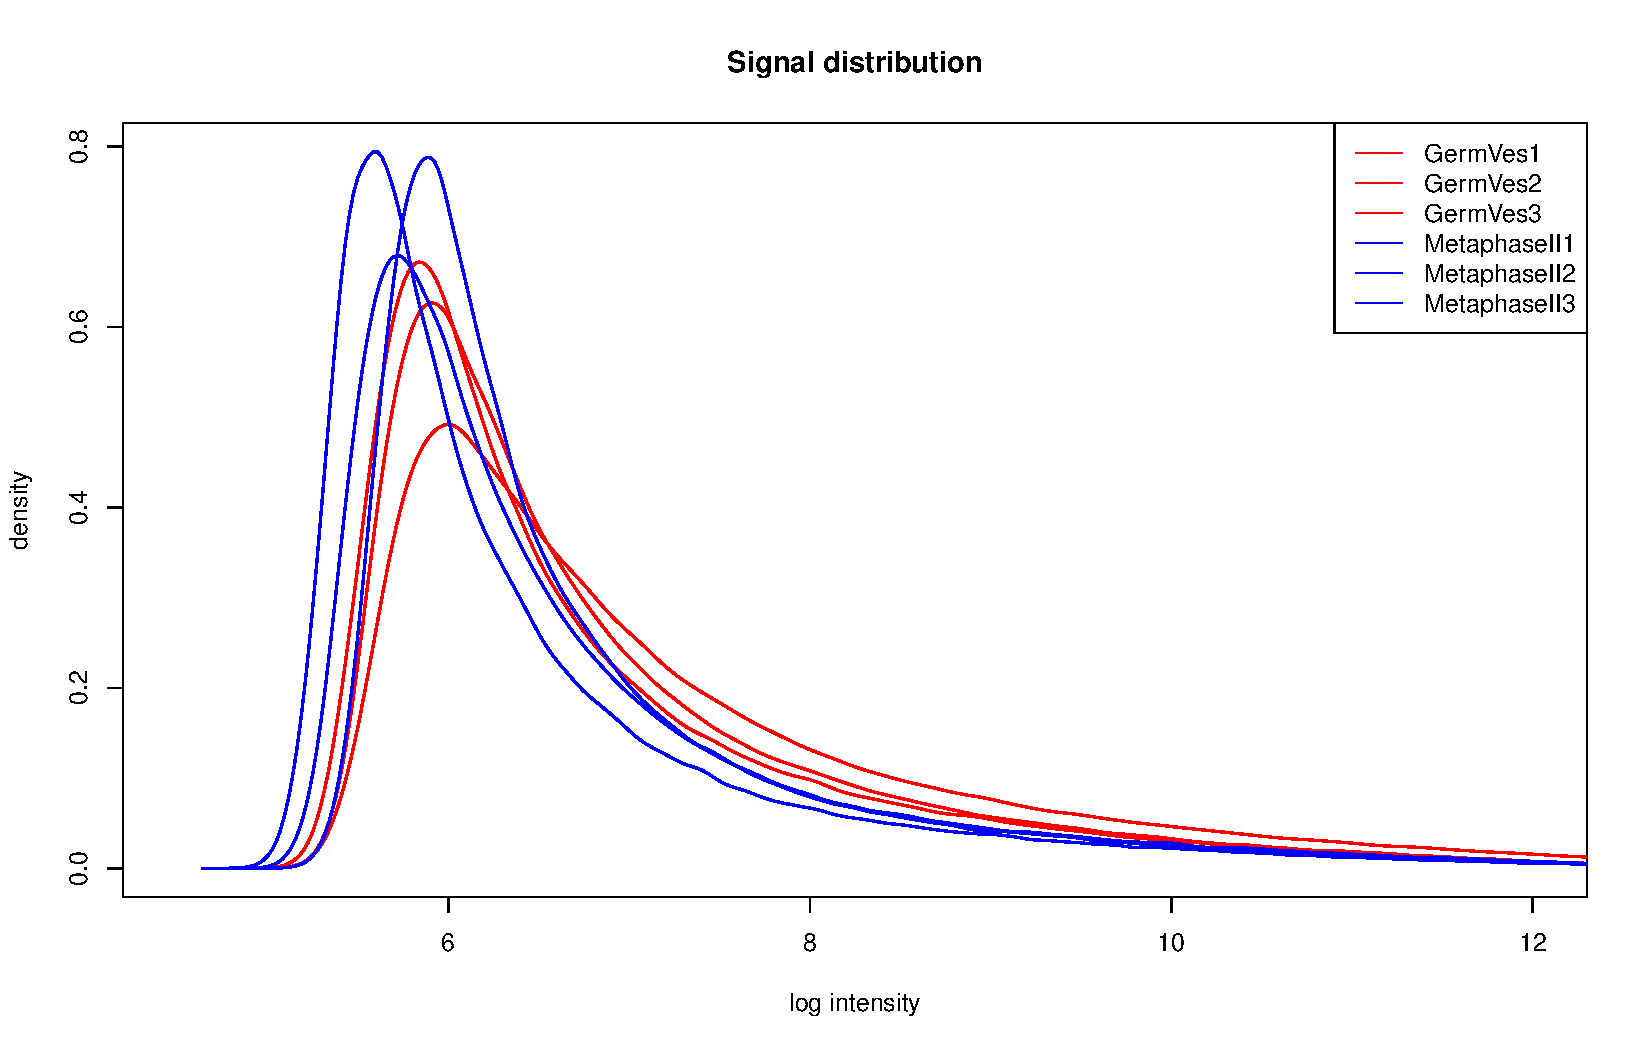
\includegraphics{Código-PEC1-Nuevo_files/figure-latex/unnamed-chunk-2-1.pdf}

\hypertarget{diagrama-de-cajas}{%
\subsubsection{Diagrama de cajas}\label{diagrama-de-cajas}}

Muestra información similar al gráfico de densidad, facilitando la
comparación entre distribuciones.

\begin{Shaded}
\begin{Highlighting}[]
\OperatorTok{>}\StringTok{ }\KeywordTok{boxplot}\NormalTok{(affy.data, }\DataTypeTok{cex.axis=}\FloatTok{0.6}\NormalTok{, }\DataTypeTok{col =}\NormalTok{ colores, }\DataTypeTok{las =} \DecValTok{2}\NormalTok{,}
\OperatorTok{+}\StringTok{         }\DataTypeTok{names =}\NormalTok{ sampleNames)}
\end{Highlighting}
\end{Shaded}

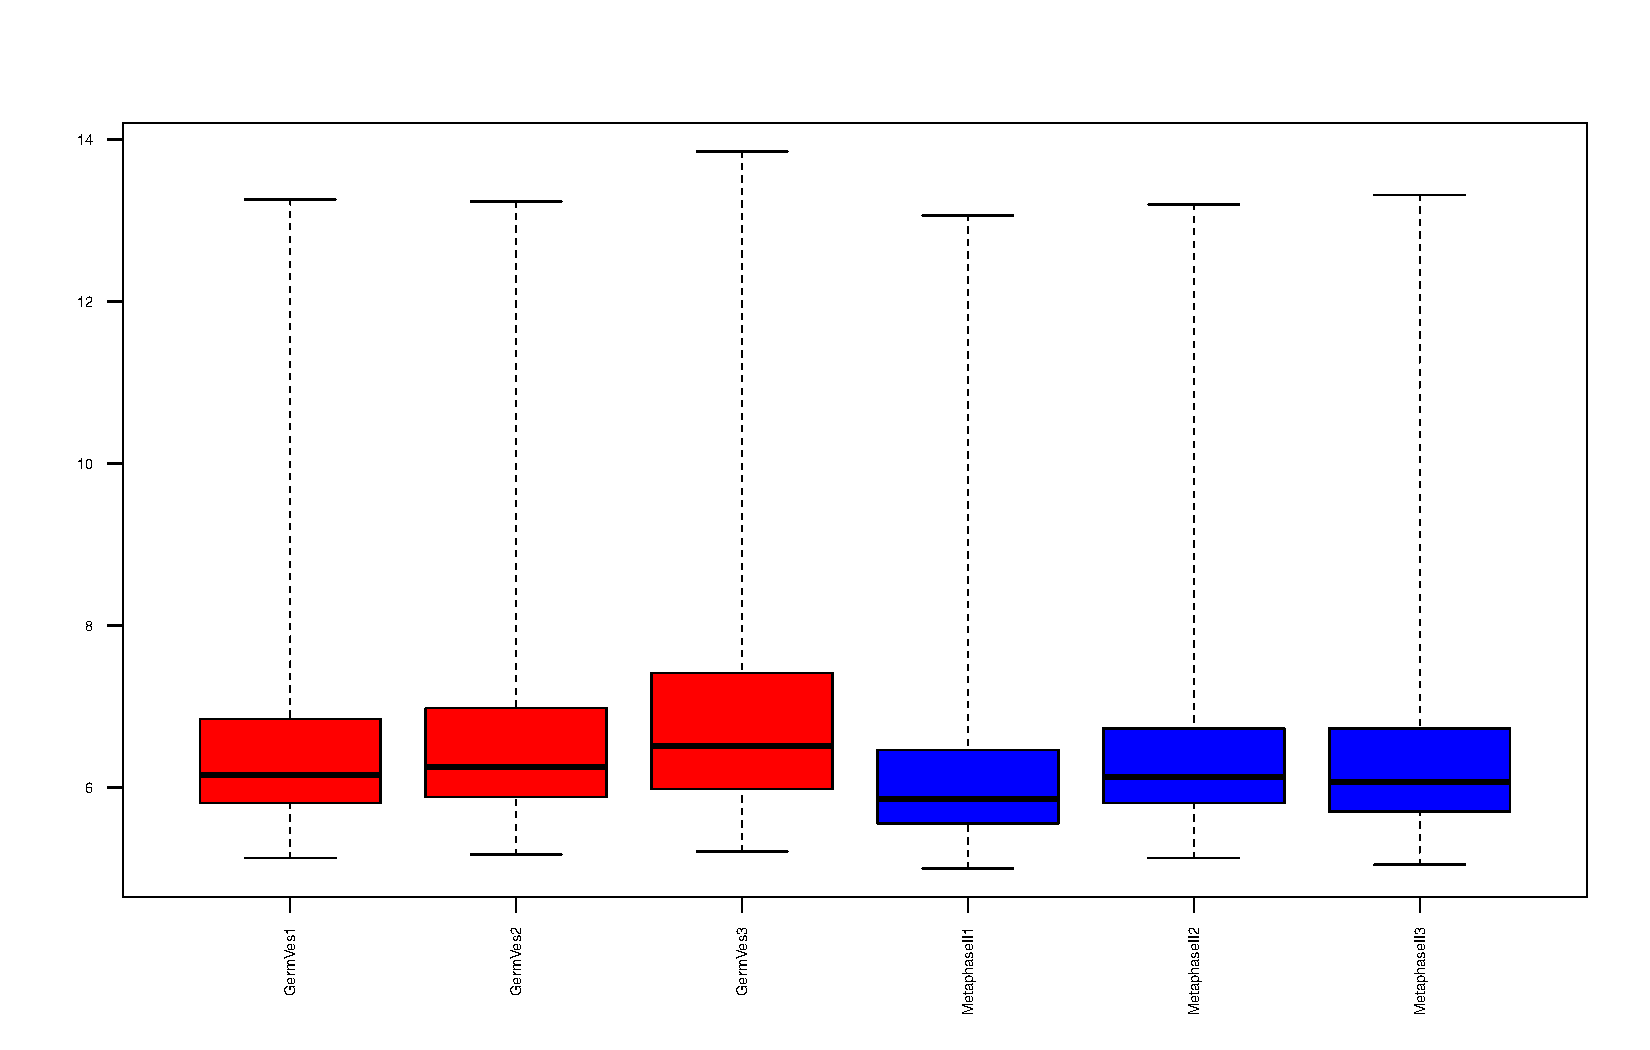
\includegraphics{Código-PEC1-Nuevo_files/figure-latex/unnamed-chunk-3-1.pdf}

\hypertarget{anuxe1lisis-de-componentes-principales-pca}{%
\subsubsection{Análisis de componentes principales
(PCA)}\label{anuxe1lisis-de-componentes-principales-pca}}

Empleando el análisis de componentes principales detectamos si las
muestras se agrupan por grupos de manera coherente (MII frente a
GermVes). El PC1 separa bastante bien los grupos, lo cual es importante
porque agrupa un porcentaje muy elevado de la varianza (73\%). El PC2
presenta agrupa un porcentaje menor de la varianza, y principalmente
separa réplicas (13.3\%). Germvers3 se aleja ligeramente del resto, pero
no creo que sea una diferencia especialmente elevada. Podemos considerar
el enfoque de PC como bueno, ya que en total, recoje el 86.3\% de la
varianza de las muestras.

\begin{Shaded}
\begin{Highlighting}[]
\OperatorTok{>}\StringTok{ }\NormalTok{logaffy <-}\StringTok{ }\KeywordTok{log2}\NormalTok{(}\KeywordTok{exprs}\NormalTok{(affy.data))}
\OperatorTok{>}\StringTok{ }\NormalTok{plotPCA <-}\StringTok{ }\ControlFlowTok{function}\NormalTok{(X, }\DataTypeTok{labels =}\NormalTok{ affy.data}\OperatorTok{$}\NormalTok{sample, }\DataTypeTok{colors =}\NormalTok{ colores, }
\OperatorTok{+}\StringTok{                       }\DataTypeTok{dataDesc =} \StringTok{""}\NormalTok{, }\DataTypeTok{scale =} \OtherTok{FALSE}\NormalTok{)}
\OperatorTok{+}\StringTok{ }\NormalTok{\{}
\OperatorTok{+}\StringTok{ }\NormalTok{pcX <-}\StringTok{ }\KeywordTok{prcomp}\NormalTok{(}\KeywordTok{t}\NormalTok{(X), }\DataTypeTok{scale =}\NormalTok{ scale)}
\OperatorTok{+}\StringTok{ }\NormalTok{loads <-}\StringTok{ }\KeywordTok{round}\NormalTok{(pcX}\OperatorTok{$}\NormalTok{sdev}\OperatorTok{^}\DecValTok{2}\OperatorTok{/}\KeywordTok{sum}\NormalTok{(pcX}\OperatorTok{$}\NormalTok{sdev}\OperatorTok{^}\DecValTok{2}\NormalTok{)}\OperatorTok{*}\DecValTok{100}\NormalTok{, }\DecValTok{1}\NormalTok{)}
\OperatorTok{+}\StringTok{ }\NormalTok{xlab <-}\StringTok{ }\KeywordTok{c}\NormalTok{(}\KeywordTok{paste}\NormalTok{(}\StringTok{"PC1"}\NormalTok{,loads[}\DecValTok{1}\NormalTok{],}\StringTok{"%"}\NormalTok{))}
\OperatorTok{+}\StringTok{ }\NormalTok{ylab <-}\StringTok{ }\KeywordTok{c}\NormalTok{(}\KeywordTok{paste}\NormalTok{(}\StringTok{"PC2"}\NormalTok{,loads[}\DecValTok{2}\NormalTok{],}\StringTok{"%"}\NormalTok{))}
\OperatorTok{+}\StringTok{ }\ControlFlowTok{if}\NormalTok{ (}\KeywordTok{is.null}\NormalTok{(colors)) colors=}\DecValTok{1}
\OperatorTok{+}\StringTok{ }\KeywordTok{plot}\NormalTok{(pcX}\OperatorTok{$}\NormalTok{x[,}\DecValTok{1}\OperatorTok{:}\DecValTok{2}\NormalTok{], }\DataTypeTok{xlab =}\NormalTok{ xlab, }\DataTypeTok{ylab =}\NormalTok{ ylab, }\DataTypeTok{col =}\NormalTok{ colors, }\DataTypeTok{pch =} \DecValTok{19}\NormalTok{,}
\OperatorTok{+}\StringTok{ }\DataTypeTok{xlim =} \KeywordTok{c}\NormalTok{(}\KeywordTok{min}\NormalTok{(pcX}\OperatorTok{$}\NormalTok{x[,}\DecValTok{1}\NormalTok{])}\OperatorTok{-}\DecValTok{10}\NormalTok{, }\KeywordTok{max}\NormalTok{(pcX}\OperatorTok{$}\NormalTok{x[,}\DecValTok{1}\NormalTok{])}\OperatorTok{+}\DecValTok{10}\NormalTok{),}
\OperatorTok{+}\StringTok{ }\DataTypeTok{ylim =} \KeywordTok{c}\NormalTok{(}\KeywordTok{min}\NormalTok{(pcX}\OperatorTok{$}\NormalTok{x[,}\DecValTok{2}\NormalTok{])}\OperatorTok{-}\DecValTok{10}\NormalTok{, }\KeywordTok{max}\NormalTok{(pcX}\OperatorTok{$}\NormalTok{x[,}\DecValTok{2}\NormalTok{])}\OperatorTok{+}\DecValTok{10}\NormalTok{),}
\OperatorTok{+}\StringTok{ }\NormalTok{)}
\OperatorTok{+}\StringTok{ }\KeywordTok{text}\NormalTok{(pcX}\OperatorTok{$}\NormalTok{x[,}\DecValTok{1}\NormalTok{], pcX}\OperatorTok{$}\NormalTok{x[,}\DecValTok{2}\NormalTok{], labels, }\DataTypeTok{pos=}\DecValTok{3}\NormalTok{, }\DataTypeTok{cex=}\FloatTok{0.8}\NormalTok{)}
\OperatorTok{+}\StringTok{ }\KeywordTok{title}\NormalTok{(}\KeywordTok{paste}\NormalTok{(}\StringTok{"Plot of first 2 PCs for expressions in"}\NormalTok{, dataDesc, }\DataTypeTok{sep=}\StringTok{" "}\NormalTok{), }\DataTypeTok{cex =} \FloatTok{0.8}\NormalTok{)}
\OperatorTok{+}\StringTok{ }\NormalTok{\}}
\OperatorTok{>}\StringTok{ }\KeywordTok{plotPCA}\NormalTok{(logaffy)}
\end{Highlighting}
\end{Shaded}

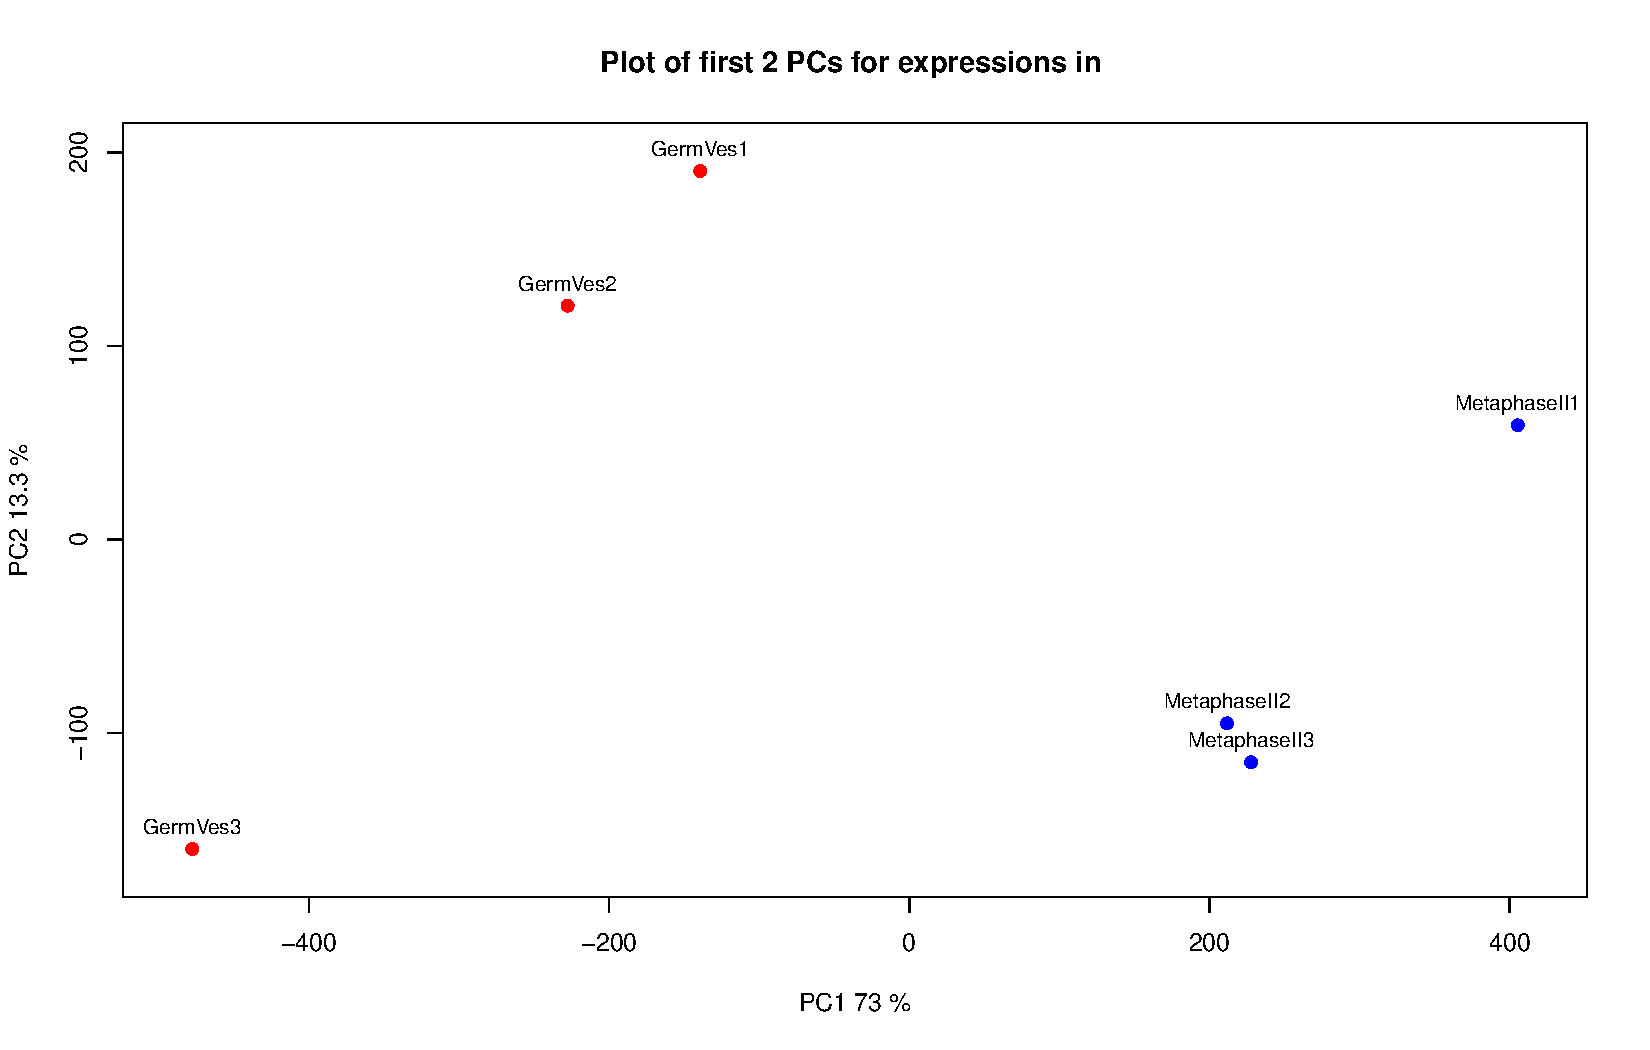
\includegraphics{Código-PEC1-Nuevo_files/figure-latex/unnamed-chunk-4-1.pdf}

\hypertarget{control-de-calidad-especuxedfico-para-microarrays}{%
\subsection{Control de calidad específico para
microarrays}\label{control-de-calidad-especuxedfico-para-microarrays}}

\hypertarget{dendrograma}{%
\subsubsection{Dendrograma}\label{dendrograma}}

Dendrograma resultante de un agrupamiento jerárquico. De nuevo,
GermVesc3 no se agrupa con las sus muestras de GermVesc, lo que puede
significar que hay cierta variación que puede deberse a procedimiento
experimental, Esta heterogeneidad de la mueestra no debería suponer un
problema mayor después de la normalización y filtraje de los datos.

\begin{Shaded}
\begin{Highlighting}[]
\OperatorTok{>}\StringTok{ }\NormalTok{clust.euclid.average <-}\StringTok{ }\KeywordTok{hclust}\NormalTok{(}\KeywordTok{dist}\NormalTok{(}\KeywordTok{t}\NormalTok{(}\KeywordTok{exprs}\NormalTok{(affy.data))), }\DataTypeTok{method =} \StringTok{"average"}\NormalTok{)}
\OperatorTok{>}\StringTok{ }\KeywordTok{plot}\NormalTok{(clust.euclid.average, }\DataTypeTok{labels =}\NormalTok{ sampleNames, }\DataTypeTok{main =} \StringTok{"Hierarchical}
\StringTok{+ clustering of samples"}\NormalTok{, }\DataTypeTok{hang =} \DecValTok{-1}\NormalTok{)}
\end{Highlighting}
\end{Shaded}

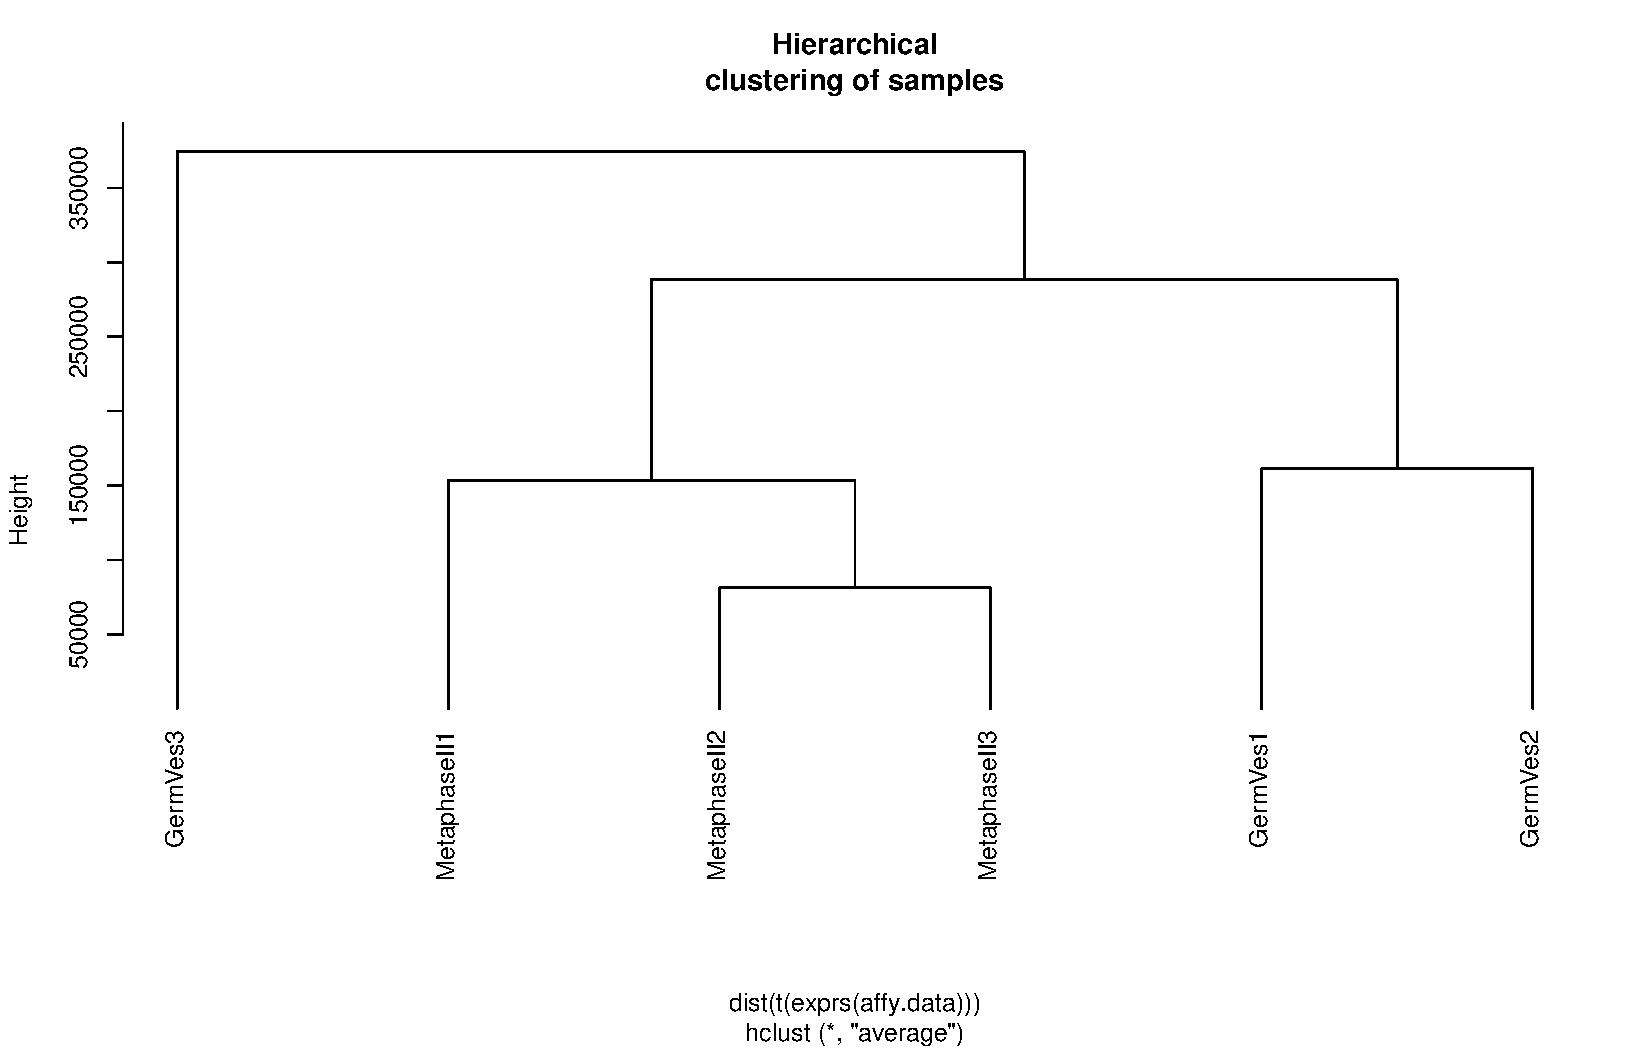
\includegraphics{Código-PEC1-Nuevo_files/figure-latex/unnamed-chunk-5-1.pdf}

\hypertarget{gruxe1fico-de-degradaciuxf3n}{%
\subsubsection{Gráfico de
degradación}\label{gruxe1fico-de-degradaciuxf3n}}

\begin{Shaded}
\begin{Highlighting}[]
\OperatorTok{>}\StringTok{ }\NormalTok{deg <-}\StringTok{ }\KeywordTok{AffyRNAdeg}\NormalTok{(affy.data)}
\OperatorTok{>}\StringTok{ }\NormalTok{cols <-}\StringTok{ }\KeywordTok{sample}\NormalTok{(}\KeywordTok{colors}\NormalTok{(), }\KeywordTok{nrow}\NormalTok{(}\KeywordTok{pData}\NormalTok{(affy.data)))}
\OperatorTok{>}\StringTok{ }\KeywordTok{plotAffyRNAdeg}\NormalTok{(deg, }\DataTypeTok{col=}\NormalTok{colores)}
\OperatorTok{>}\StringTok{ }\KeywordTok{legend}\NormalTok{(}\DataTypeTok{legend =} \KeywordTok{sampleNames}\NormalTok{(affy.data), }\DataTypeTok{x =} \StringTok{"topleft"}\NormalTok{, }\DataTypeTok{lty =} \DecValTok{1}\NormalTok{, }\DataTypeTok{col =}\NormalTok{ colores)}
\end{Highlighting}
\end{Shaded}

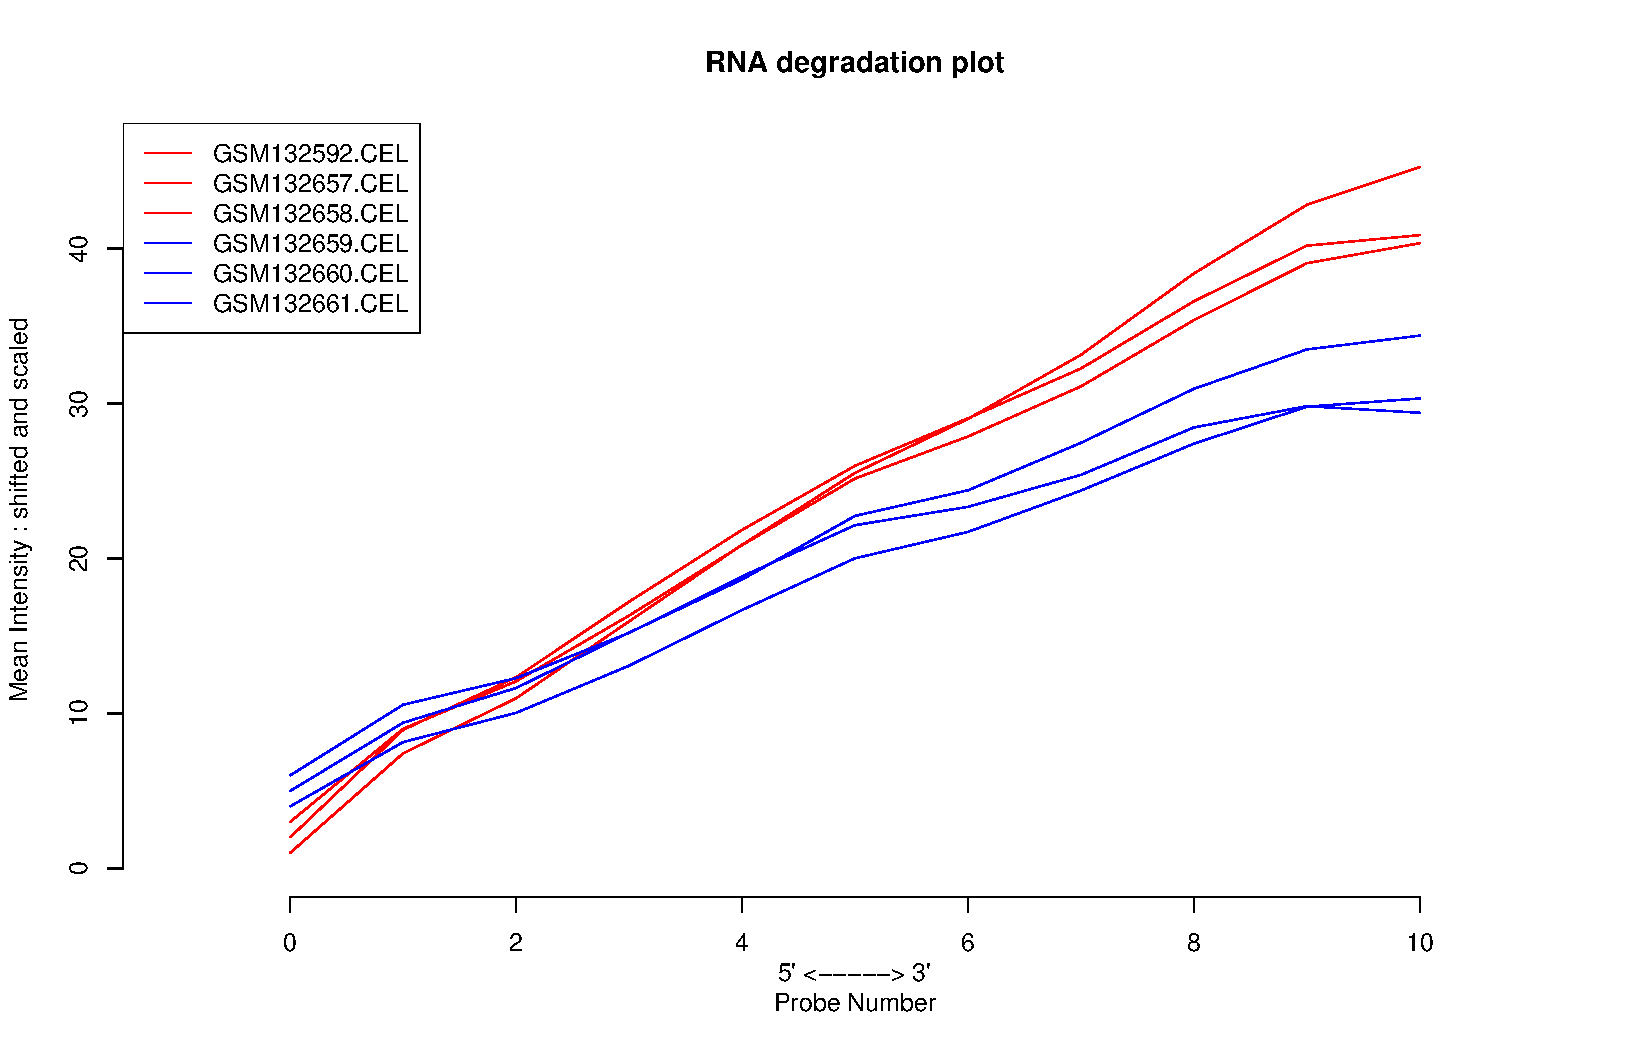
\includegraphics{Código-PEC1-Nuevo_files/figure-latex/unnamed-chunk-6-1.pdf}

\hypertarget{gruxe1fico-de-expresiones-relativas-rle}{%
\subsubsection{Gráfico de expresiones relativas
(RLE)}\label{gruxe1fico-de-expresiones-relativas-rle}}

Gráfico de expresiones relativas (RLE) resultante del análisis basado en
modelos (PLM). Las muestras son simétricas y similares lo que sugiera
una calidad aceptable de los datos

\begin{Shaded}
\begin{Highlighting}[]
\OperatorTok{>}\StringTok{ }\NormalTok{computePLM <-}\StringTok{ }\NormalTok{T}
\OperatorTok{>}\StringTok{ }\ControlFlowTok{if}\NormalTok{(computePLM)\{}
\OperatorTok{+}\StringTok{ }\NormalTok{Pset <-}\StringTok{ }\KeywordTok{fitPLM}\NormalTok{(affy.data)}
\OperatorTok{+}\StringTok{ }\KeywordTok{save}\NormalTok{(Pset, }\DataTypeTok{file =} \KeywordTok{file.path}\NormalTok{(workingdir,}\StringTok{"PLM.Rda"}\NormalTok{))}
\OperatorTok{+}\StringTok{ }\NormalTok{\}}\ControlFlowTok{else}\NormalTok{\{}
\OperatorTok{+}\StringTok{ }\KeywordTok{load}\NormalTok{ (}\DataTypeTok{file =} \KeywordTok{file.path}\NormalTok{(workingdir,}\StringTok{"PLM.Rda"}\NormalTok{))}
\OperatorTok{+}\StringTok{ }\NormalTok{\}}
\OperatorTok{>}\StringTok{ }\KeywordTok{RLE}\NormalTok{(Pset, }\DataTypeTok{main =} \StringTok{"Relative Log Expression"}\NormalTok{, }\DataTypeTok{names =}\NormalTok{ sampleNames,}
\OperatorTok{+}\StringTok{ }\DataTypeTok{las =} \DecValTok{2}\NormalTok{, }\DataTypeTok{col =}\NormalTok{ colores, }\DataTypeTok{cex.axis =} \FloatTok{0.6}\NormalTok{, }\DataTypeTok{ylim =} \KeywordTok{c}\NormalTok{(}\OperatorTok{-}\DecValTok{5}\NormalTok{,}\DecValTok{5}\NormalTok{))}
\end{Highlighting}
\end{Shaded}

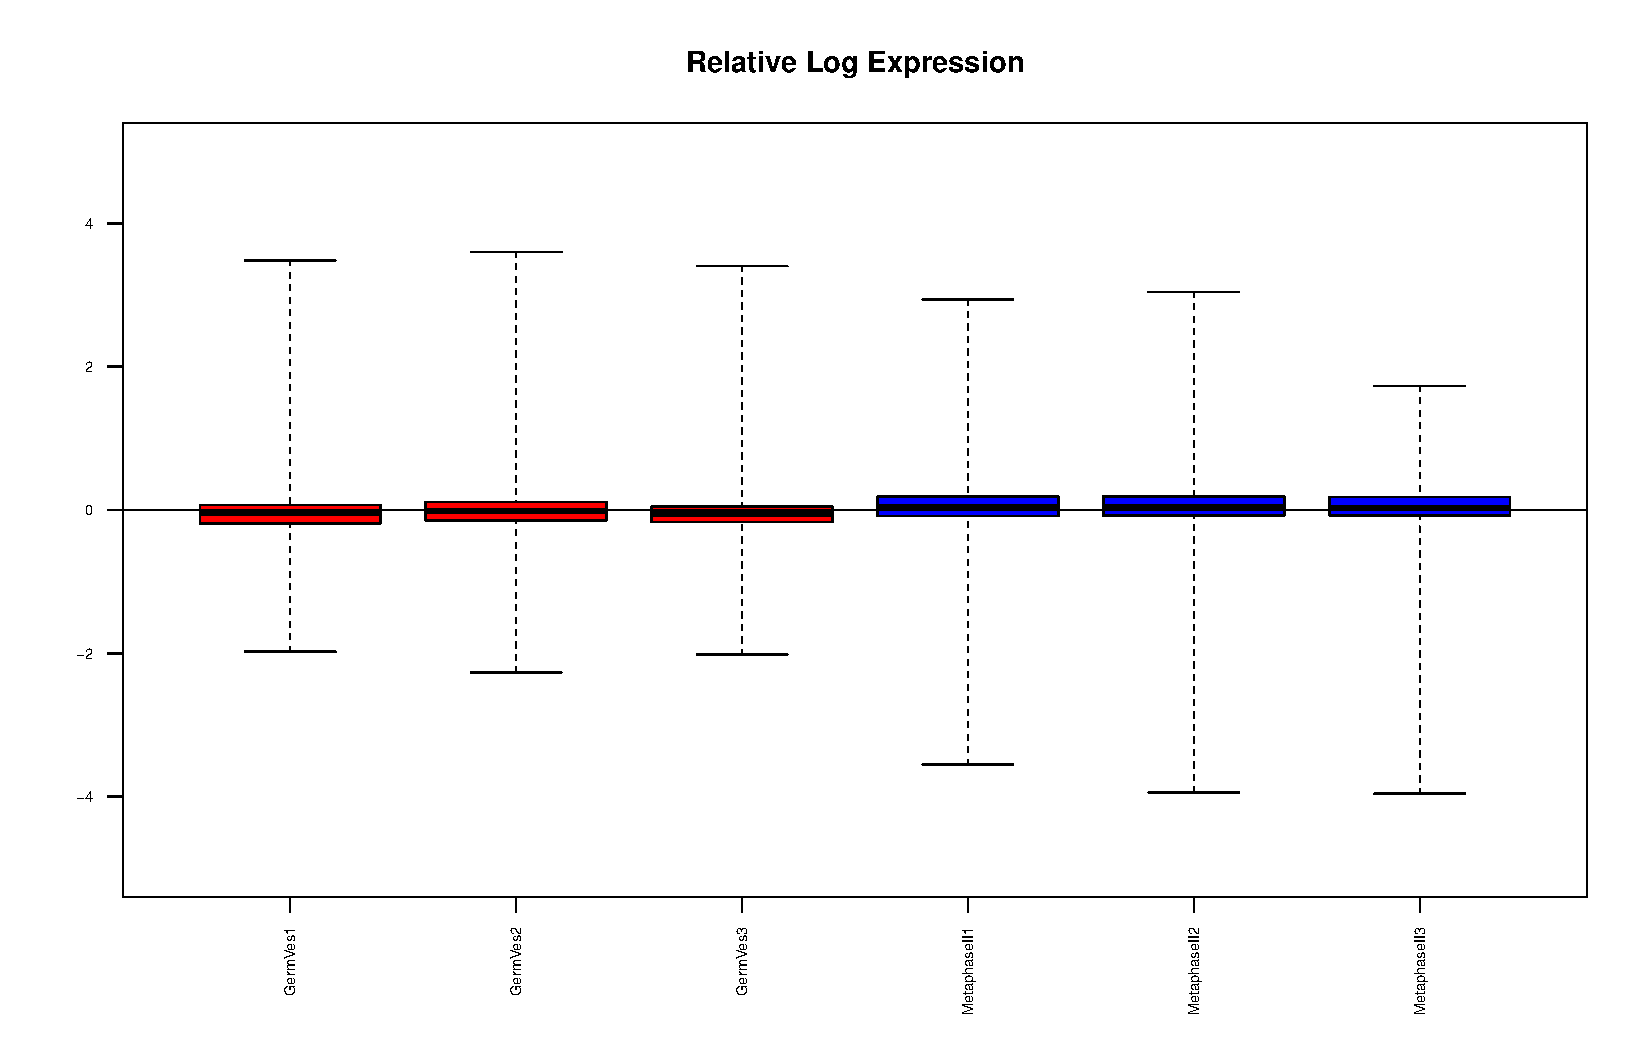
\includegraphics{Código-PEC1-Nuevo_files/figure-latex/unnamed-chunk-7-1.pdf}

\hypertarget{normalizaciuxf3n}{%
\section{Normalización}\label{normalizaciuxf3n}}

Mediante la normalización por RMA (robust multi-array average) se
corregirá el background de los arrays y se transformarán los datos
utilizando el logaritmo en base 2 de cada intensidad ajustada. El método
de normalización por RMA se basa en los distintos valores de las sondas
para un mismo gen en cada uno de los chips de microarrays. Las sondas de
menor intensidad tienen variaciones de intensidad que se aproximan a 0,
por lo que al usar RMA no se debería necesitar realizar un filtraje
no-específico. El filtraje no específico podría introducir sesgos en
nuestros datos al afectar el comportamiento en los análisis posteriores,
sin embargo, posteriormente realizaremos un filtraje no específico y
compararemos el output del procesado de los dos conjuntos de datos.

En el boxplot de los valores normalizados se observa que los valores en
una situación que permite su comparación

\begin{Shaded}
\begin{Highlighting}[]
\OperatorTok{>}\StringTok{ }\NormalTok{ovo <-}\StringTok{ }\KeywordTok{rma}\NormalTok{(affy.data)}
\end{Highlighting}
\end{Shaded}

\begin{verbatim}
Background correcting
Normalizing
Calculating Expression
\end{verbatim}

\begin{Shaded}
\begin{Highlighting}[]
\OperatorTok{>}\StringTok{ }\NormalTok{ovo.rma <-}\StringTok{ }\KeywordTok{exprs}\NormalTok{(ovo)}
\OperatorTok{>}\StringTok{ }\KeywordTok{boxplot}\NormalTok{(ovo.rma,}\DataTypeTok{main=}\StringTok{"Boxplot for RMA-normalized expression values"}\NormalTok{,}
\OperatorTok{+}\StringTok{ }\DataTypeTok{names =}\NormalTok{ sampleNames, }\DataTypeTok{cex.axis =} \FloatTok{0.7}\NormalTok{, }\DataTypeTok{col =}\NormalTok{ colores,}\DataTypeTok{las =} \DecValTok{2}\NormalTok{)}
\end{Highlighting}
\end{Shaded}

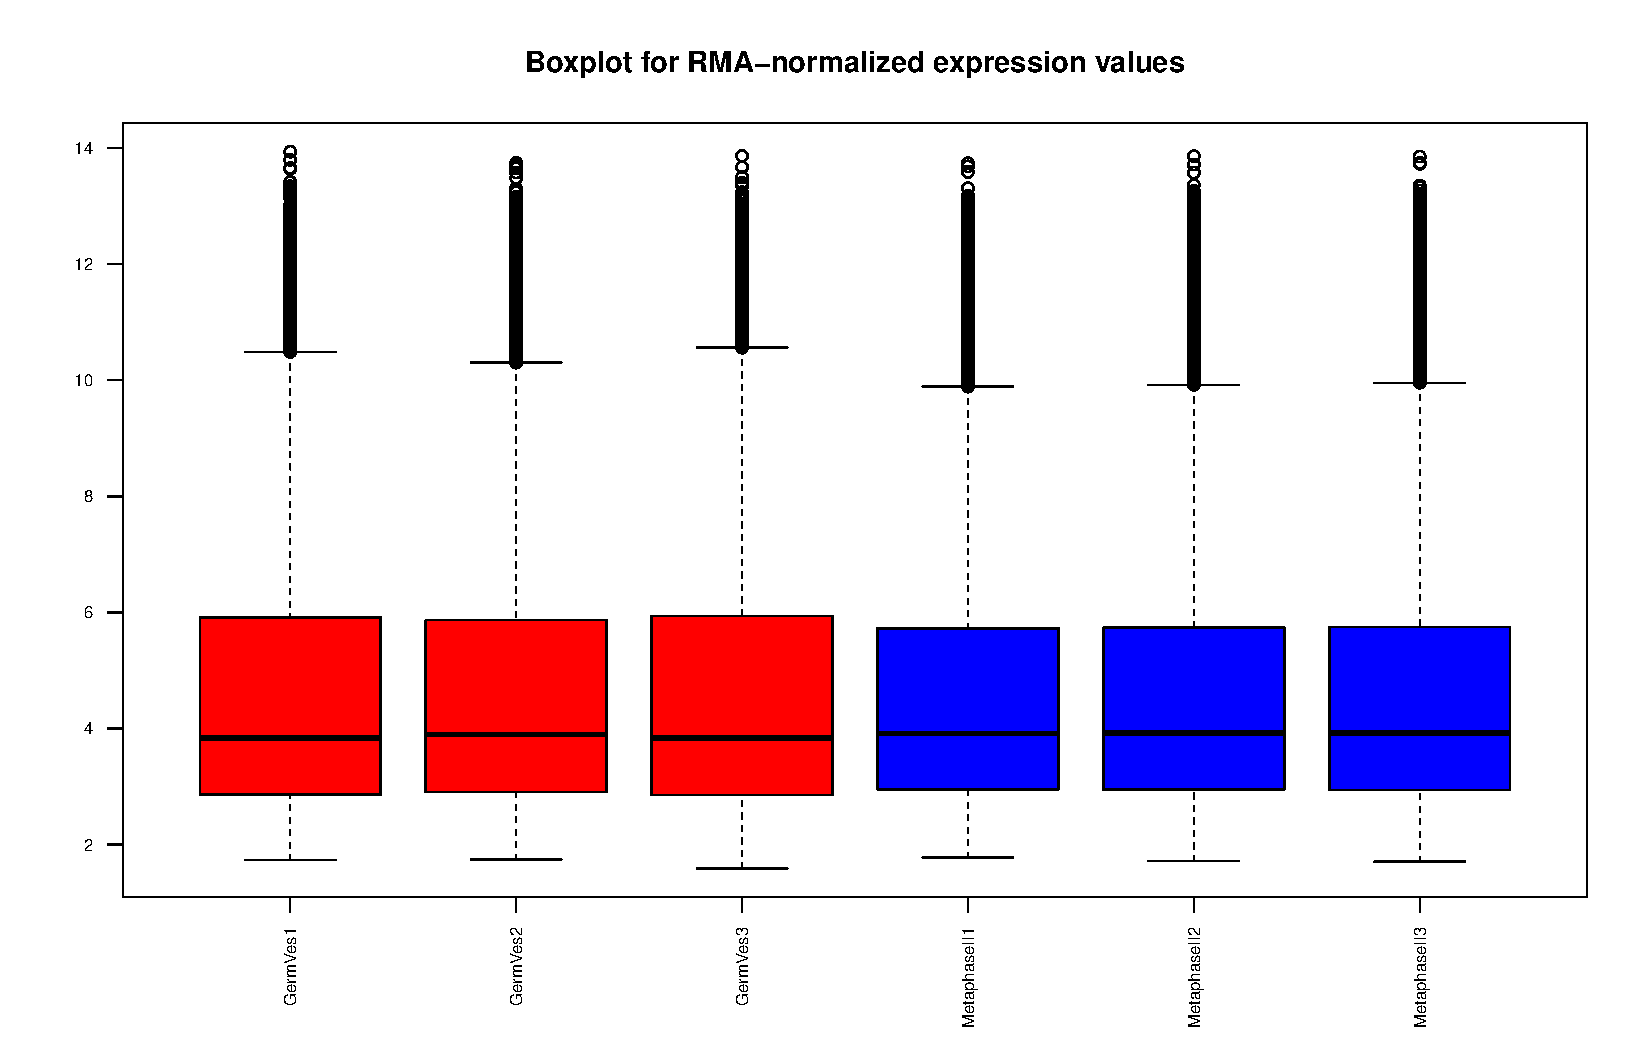
\includegraphics{Código-PEC1-Nuevo_files/figure-latex/unnamed-chunk-8-1.pdf}

\begin{Shaded}
\begin{Highlighting}[]
\OperatorTok{>}\StringTok{ }\KeywordTok{colnames}\NormalTok{(ovo.rma) <-}\StringTok{ }\KeywordTok{c}\NormalTok{(}\StringTok{"GermVes1"}\NormalTok{,}\StringTok{"GermVes2"}\NormalTok{,}\StringTok{"GermVes3"}\NormalTok{,}\StringTok{"MII1"}\NormalTok{,}\StringTok{"MII2"}\NormalTok{,}\StringTok{"MII3"}\NormalTok{)}
\OperatorTok{>}\StringTok{ }\KeywordTok{dim}\NormalTok{(ovo.rma)}
\end{Highlighting}
\end{Shaded}

\begin{verbatim}
[1] 45101     6
\end{verbatim}

\hypertarget{selecciuxf3n-de-genes-con-expresiuxf3n-diferencial}{%
\section{Selección de genes con expresión
diferencial}\label{selecciuxf3n-de-genes-con-expresiuxf3n-diferencial}}

\hypertarget{matriz-de-diseuxf1o-y-matriz-de-contraste}{%
\subsection{Matriz de diseño y matriz de
contraste}\label{matriz-de-diseuxf1o-y-matriz-de-contraste}}

La matriz de diseño aporta asignación de cada muestra a un grupo (cada
fila contiene un uno en la columna del grupo y cero en el resto)

La matriz de contrastes describe las comparaciones entre grupos. En este
caso la matriz de comparación es muy simple, pero de forma habitual
consta de tantas columnas como comparaciones y filas como grupos.

\begin{Shaded}
\begin{Highlighting}[]
\OperatorTok{>}\StringTok{ }\NormalTok{design <-}\StringTok{ }\KeywordTok{matrix}\NormalTok{(}\KeywordTok{c}\NormalTok{(}\DecValTok{1}\NormalTok{,}\DecValTok{1}\NormalTok{,}\DecValTok{1}\NormalTok{,}\DecValTok{0}\NormalTok{,}\DecValTok{0}\NormalTok{,}\DecValTok{0}\NormalTok{,}\DecValTok{0}\NormalTok{,}\DecValTok{0}\NormalTok{,}\DecValTok{0}\NormalTok{,}\DecValTok{1}\NormalTok{,}\DecValTok{1}\NormalTok{,}\DecValTok{1}\NormalTok{), }\DataTypeTok{nrow=}\DecValTok{6}\NormalTok{)}
\OperatorTok{>}\StringTok{ }\KeywordTok{colnames}\NormalTok{(design) <-}\StringTok{ }\KeywordTok{c}\NormalTok{(}\StringTok{"GermVes"}\NormalTok{, }\StringTok{"Metaphase"}\NormalTok{)}
\OperatorTok{>}\StringTok{ }\KeywordTok{rownames}\NormalTok{(design) <-}\StringTok{ }\KeywordTok{c}\NormalTok{(}\StringTok{"GermVes1"}\NormalTok{, }\StringTok{"GermVes2"}\NormalTok{, }\StringTok{"GermVes3"}\NormalTok{, }\StringTok{"MII1"}\NormalTok{, }\StringTok{"MII2"}\NormalTok{,   }\StringTok{"MII3"}\NormalTok{)}
\OperatorTok{>}\StringTok{ }\NormalTok{design}
\end{Highlighting}
\end{Shaded}

\begin{verbatim}
         GermVes Metaphase
GermVes1       1         0
GermVes2       1         0
GermVes3       1         0
MII1           0         1
MII2           0         1
MII3           0         1
\end{verbatim}

\begin{Shaded}
\begin{Highlighting}[]
\OperatorTok{>}\StringTok{ }\NormalTok{cont.matrix <-}\StringTok{ }\KeywordTok{makeContrasts}\NormalTok{ (}\DataTypeTok{MetaphaseII =}\NormalTok{ (Metaphase}\OperatorTok{-}\NormalTok{GermVes), }\DataTypeTok{levels=}\NormalTok{design)}
\OperatorTok{>}\StringTok{ }\NormalTok{cont.matrix}
\end{Highlighting}
\end{Shaded}

\begin{verbatim}
           Contrasts
Levels      MetaphaseII
  GermVes            -1
  Metaphase           1
\end{verbatim}

\hypertarget{estimaciuxf3n-del-modelo-y-selecciuxf3n-de-genes}{%
\subsection{Estimación del modelo y selección de
genes}\label{estimaciuxf3n-del-modelo-y-selecciuxf3n-de-genes}}

Generamos el modelo lineal a partir de los datos normalizados y las
matrices. En \emph{limma} amplía el análisis empleando modelos de Bayes
empíricos, combinando información la matriz de datos y de cada gen
individual, lo que obtiene estimaciones de error mejoradas. Para
controlar el porcentaje de falsos positivos, los p-valores se ajustan
utilizando el metodo de Benjamini y Hochberg.

Como método de visualización, con el volcanoplot podemos apreciar los
genes más interesantes (log2 Fold Change neto elevado para la
significación biológica y −log10(P−value) elevado para la estadística)

En el gráfico, podemos la asimetría hacia la izquierda, lo que indica un
menor número genes transcripcionalmente activos en metafase II
comparados con el estadio de vesícula germinal. Esto es coherente ya que
en Metafase II, la heterocromatina está compactada formando la placa
metafásica ecuatorial, siendo esta apenas accesible a la maquinaria de
transcripción.

\begin{Shaded}
\begin{Highlighting}[]
\OperatorTok{>}\StringTok{ }\NormalTok{fit <-}\StringTok{ }\KeywordTok{lmFit}\NormalTok{(ovo.rma, design)}
\OperatorTok{>}\StringTok{ }\NormalTok{fit.main <-}\StringTok{ }\KeywordTok{contrasts.fit}\NormalTok{(fit, cont.matrix)}
\OperatorTok{>}\StringTok{ }\NormalTok{fit.main <-}\StringTok{ }\KeywordTok{eBayes}\NormalTok{(fit.main)}
\OperatorTok{>}\StringTok{ }\NormalTok{topTabMII <-}\StringTok{ }\KeywordTok{topTable}\NormalTok{ (fit.main, }\DataTypeTok{number =} \KeywordTok{nrow}\NormalTok{(fit.main), }\DataTypeTok{coef =} \StringTok{"MetaphaseII"}\NormalTok{, }\DataTypeTok{adjust=}\StringTok{"fdr"}\NormalTok{)}
\OperatorTok{>}\StringTok{ }\NormalTok{coefnum=}\DecValTok{1}
\OperatorTok{>}\StringTok{ }\KeywordTok{volcanoplot}\NormalTok{(fit.main, }\DataTypeTok{coef =} \DecValTok{1}\NormalTok{, }\DataTypeTok{highlight =} \DecValTok{10}\NormalTok{, }\DataTypeTok{names =}\NormalTok{ exprs}\OperatorTok{$}\NormalTok{Gene.symbol ,}
\OperatorTok{+}\StringTok{             }\DataTypeTok{style=} \StringTok{"p-value"}\NormalTok{, }\DataTypeTok{main =} \StringTok{"Differentially expressed genes"}\NormalTok{)}
\OperatorTok{>}\StringTok{ }\KeywordTok{abline}\NormalTok{(}\DataTypeTok{v =} \KeywordTok{c}\NormalTok{(}\OperatorTok{-}\DecValTok{2}\NormalTok{,}\DecValTok{2}\NormalTok{))}
\end{Highlighting}
\end{Shaded}

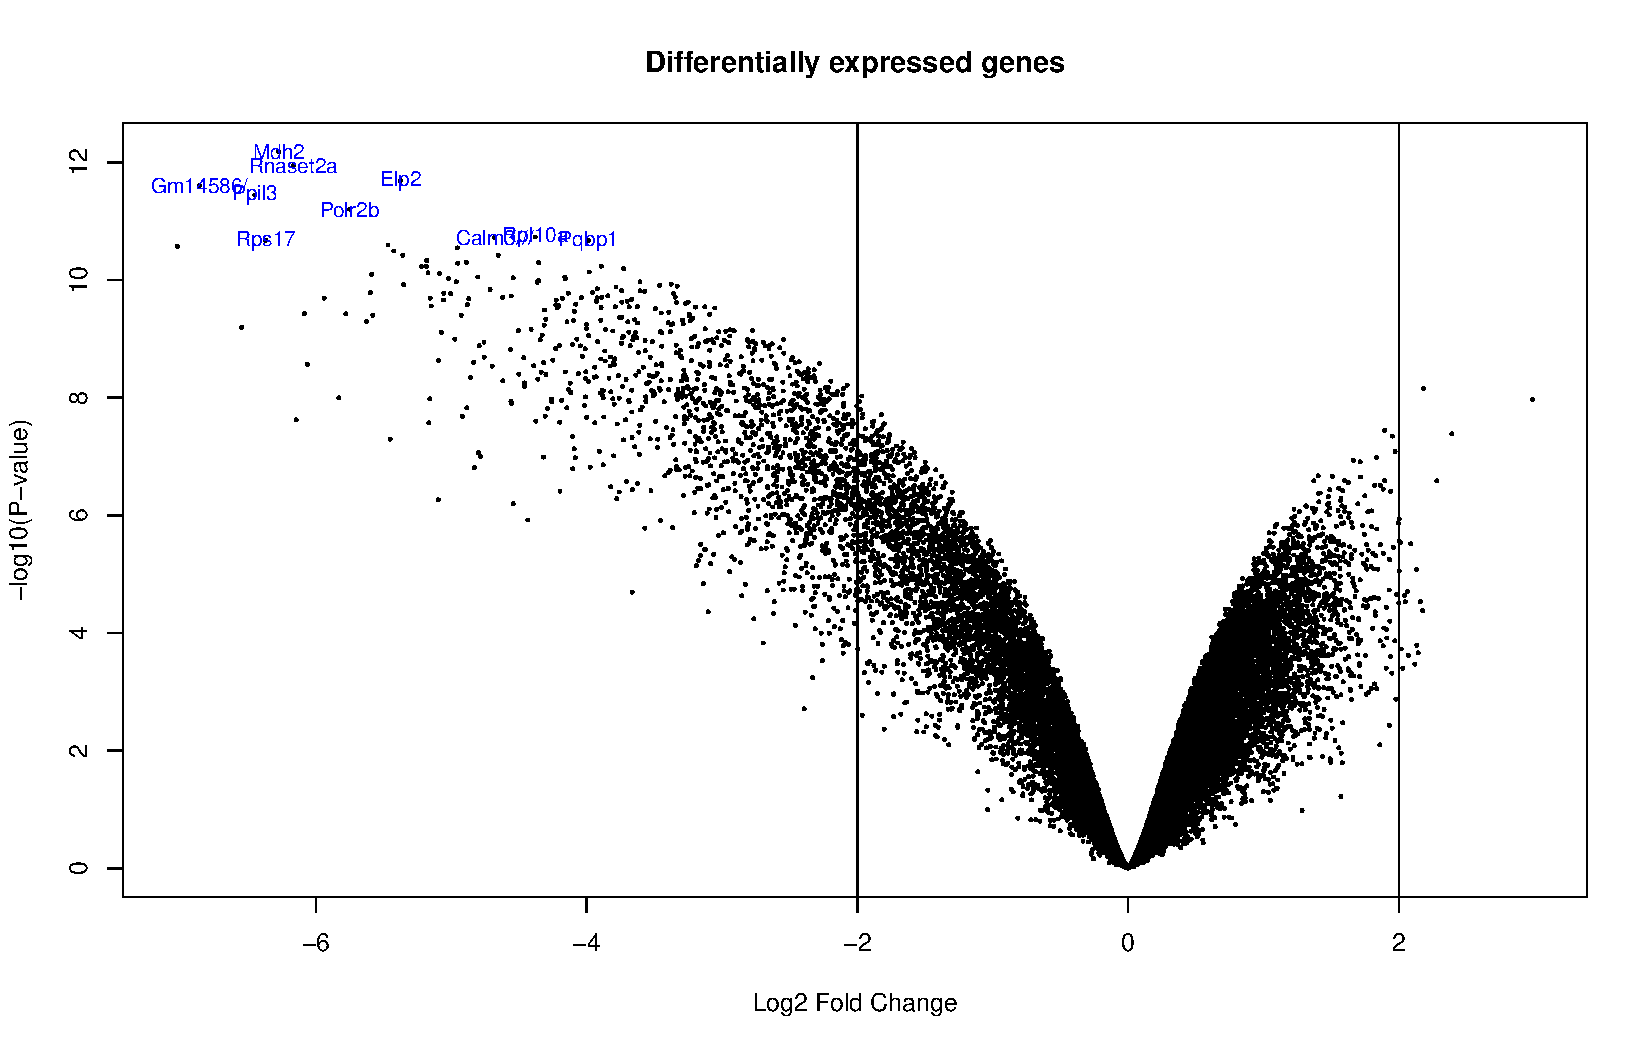
\includegraphics{Código-PEC1-Nuevo_files/figure-latex/unnamed-chunk-10-1.pdf}

\hypertarget{principales-genes-expresados-diferencialmente}{%
\subsection{Principales genes expresados
diferencialmente}\label{principales-genes-expresados-diferencialmente}}

Para ver con más detalle los genes más relevantes, podría analizarse la
tabla \textbf{topTabMII2 } que se crea a continuación.

\begin{Shaded}
\begin{Highlighting}[]
\OperatorTok{>}\StringTok{ }\NormalTok{topTabMII2 <-}\StringTok{ }\KeywordTok{topTable}\NormalTok{ (fit.main, }\DataTypeTok{number=}\KeywordTok{nrow}\NormalTok{(fit.main), }\DataTypeTok{adjust=}\StringTok{"fdr"}\NormalTok{, }\DataTypeTok{genelist =}\NormalTok{ exprs)}
\OperatorTok{>}\StringTok{ }\KeywordTok{colnames}\NormalTok{(topTabMII2)}
\end{Highlighting}
\end{Shaded}

\begin{verbatim}
 [1] "IDENTIFIER"            "GSM132592"             "GSM132657"            
 [4] "GSM132658"             "GSM132659"             "GSM132660"            
 [7] "GSM132661"             "Gene.title"            "Gene.symbol"          
[10] "Gene.ID"               "UniGene.title"         "UniGene.symbol"       
[13] "UniGene.ID"            "Nucleotide.Title"      "GI"                   
[16] "GenBank.Accession"     "Platform_CLONEID"      "Platform_ORF"         
[19] "Platform_SPOTID"       "Chromosome.location"   "Chromosome.annotation"
[22] "GO.Function"           "GO.Process"            "GO.Component"         
[25] "GO.Function.ID"        "GO.Process.ID"         "GO.Component.ID"      
[28] "logFC"                 "AveExpr"               "t"                    
[31] "P.Value"               "adj.P.Val"             "B"                    
\end{verbatim}

\begin{Shaded}
\begin{Highlighting}[]
\OperatorTok{>}\StringTok{ }\KeywordTok{str}\NormalTok{(topTabMII2)}
\end{Highlighting}
\end{Shaded}

\begin{verbatim}
'data.frame':   45101 obs. of  33 variables:
 $ IDENTIFIER           : Factor w/ 26682 levels "","--Control",..: 18067 21851 13027 14537 20737 20646 21983 10112 22039 20842 ...
 $ GSM132592            : Factor w/ 7079 levels "","1.85027","1.88006",..: 128 399 448 343 129 310 254 361 371 6462 ...
 $ GSM132657            : Factor w/ 7079 levels "","1.85027","1.88006",..: 102 402 447 365 182 339 237 362 393 6457 ...
 $ GSM132658            : Factor w/ 7079 levels "","1.85027","1.88006",..: 82 393 446 334 83 304 204 351 369 6379 ...
 $ GSM132659            : Factor w/ 7079 levels "","1.85027","1.88006",..: 2287 4464 5812 3215 2334 3976 4748 5148 4022 2862 ...
 $ GSM132660            : Factor w/ 7079 levels "","1.85027","1.88006",..: 2230 4357 5730 3292 2317 4131 4771 5327 3662 2651 ...
 $ GSM132661            : Factor w/ 7079 levels "","1.85027","1.88006",..: 2401 4216 5742 3148 1968 3836 4794 5147 4187 2871 ...
 $ Gene.title           : Factor w/ 21709 levels "","1-acylglycerol-3-phosphate O-acyltransferase 1 (lysophosphatidic acid acyltransferase, alpha)",..: 8902 13884 4611 11930 10975 11545 13906 1847 13953 11514 ...
 $ Gene.symbol          : Factor w/ 21723 levels "","0610005C13Rik",..: 13048 16863 7897 9421 15742 15651 16998 4957 17055 15848 ...
 $ Gene.ID              : Factor w/ 21723 levels "","100008567",..: 5304 31 14083 200 17062 9118 6408 2841 6430 13411 ...
 $ UniGene.title        : Factor w/ 223 levels "","2-cell-stage, variable group, member 3",..: 1 1 1 1 1 1 1 1 1 1 ...
 $ UniGene.symbol       : Factor w/ 106 levels "","1700023F02Rik",..: 1 1 1 1 1 1 1 1 1 1 ...
 $ UniGene.ID           : Factor w/ 1792 levels "","Mm.100895",..: 1 1 1 1 1 1 1 1 1 1 ...
 $ Nucleotide.Title     : Factor w/ 36271 levels "","0104-78 Mouse E14.5 retina lambda ZAP II Library Mus musculus cDNA, mRNA sequence",..: 1493 1943 6318 11633 12728 34858 20607 23531 29706 4636 ...
 $ GI                   : int  4793932 5249372 8848789 16107822 7182938 20352496 12832724 18204695 134053886 8202382 ...
 $ GenBank.Accession    : Factor w/ 36278 levels "","AA014267",..: 7072 7522 13263 18578 10604 29704 2398 21143 31451 11581 ...
 $ Platform_CLONEID     : logi  NA NA NA NA NA NA ...
 $ Platform_ORF         : logi  NA NA NA NA NA NA ...
 $ Platform_SPOTID      : Factor w/ 2 levels "","--Control": 1 1 1 1 1 1 1 1 1 1 ...
 $ Chromosome.location  : Factor w/ 4951 levels "","1","1 1.65 cM",..: 3415 2049 2171 4869 276 3491 2038 4125 4184 4730 ...
 $ Chromosome.annotation: Factor w/ 19373 levels "","Chromosome 1",..: 13245 7967 8115 19091 820 13875 7389 15711 16483 19271 ...
 $ GO.Function          : Factor w/ 9802 levels "","(-)-E-beta-caryophyllene synthase activity///(E)-beta-ocimene synthase activity///alpha-humulene synthase activ"| __truncated__,..: 7285 8835 3881 8385 7152 4455 9063 987 8385 8578 ...
 $ GO.Process           : Factor w/ 12040 levels "","'de novo' actin filament nucleation///Arp2/3 complex-mediated actin nucleation///DNA repair///actin polymerizat"| __truncated__,..: 9459 1 10966 6987 11414 11816 8949 7743 6987 11290 ...
 $ GO.Component         : Factor w/ 9470 levels "","3-methylcrotonyl-CoA carboxylase complex, mitochondrial///mitochondrial inner membrane///mitochondrial matrix//"| __truncated__,..: 6507 5893 5869 5719 1591 5786 4553 4980 5719 2932 ...
 $ GO.Function.ID       : Factor w/ 9802 levels "","contributes_to GO:0000213",..: 7411 2908 10 8584 6740 1345 2017 5663 8584 5526 ...
 $ GO.Process.ID        : Factor w/ 12040 levels "","GO:0000002///GO:0006412",..: 2326 1 9939 8675 5810 1766 322 106 8675 5762 ...
 $ GO.Component.ID      : Factor w/ 9470 levels "","colocalizes_with GO:0000502",..: 8850 3548 7830 6502 9043 1203 2780 2824 6502 4551 ...
 $ logFC                : num  -6.27 -6.17 -5.37 -6.86 -6.45 ...
 $ AveExpr              : num  7.06 9 10.47 8.15 7.06 ...
 $ t                    : num  -63 -59.1 -55.3 -54.1 -51.9 ...
 $ P.Value              : num  6.60e-13 1.15e-12 2.06e-12 2.50e-12 3.61e-12 ...
 $ adj.P.Val            : num  2.60e-08 2.60e-08 2.82e-08 2.82e-08 3.26e-08 ...
 $ B                    : num  19.2 18.8 18.4 18.3 18 ...
\end{verbatim}

\begin{Shaded}
\begin{Highlighting}[]
\OperatorTok{>}\StringTok{ }\NormalTok{topTabMII2[}\DecValTok{1}\OperatorTok{:}\DecValTok{10}\NormalTok{,}\KeywordTok{c}\NormalTok{(}\DecValTok{28}\OperatorTok{:}\DecValTok{33}\NormalTok{)]}
\end{Highlighting}
\end{Shaded}

\begin{verbatim}
                 logFC   AveExpr         t      P.Value    adj.P.Val        B
1433984_a_at -6.274365  7.061497 -63.04831 6.601710e-13 2.599082e-08 19.20462
1456012_x_at -6.165310  9.002740 -59.13856 1.152561e-12 2.599082e-08 18.84512
1438179_s_at -5.374540 10.474811 -55.30899 2.063817e-12 2.817216e-08 18.44886
1437510_x_at -6.858772  8.152061 -54.10693 2.498584e-12 2.817216e-08 18.31438
1429627_at   -6.450413  7.057122 -51.86092 3.612891e-12 3.258900e-08 18.04887
1433552_a_at -5.749902  8.466528 -48.67839 6.266436e-12 4.710376e-08 17.63789
1431177_a_at -4.378015  8.585689 -42.94001 1.863800e-11 9.613540e-08 16.77589
1423807_a_at -4.679136  9.391626 -42.85470 1.896275e-11 9.613540e-08 16.76174
1459986_a_at -6.370147  8.711593 -42.31275 2.117900e-11 9.613540e-08 16.67082
1456086_x_at -3.984745  6.347380 -42.28144 2.131558e-11 9.613540e-08 16.66552
\end{verbatim}

\hypertarget{post-procesado-de-las-listas-de-genes-obtenidas}{%
\section{Post-procesado de las listas de genes
obtenidas}\label{post-procesado-de-las-listas-de-genes-obtenidas}}

Pueden ejecutarse diferentes tipos de análisis, encaminados a facilitar
la interpretación. En este grupo se encuentran, entre otras:

\begin{itemize}
\tightlist
\item
  La anotación de las listas de genes en diversas bases de datos.
\item
  La comparación entre las listas para determinar qué genes cambian
  simultaneamente en varias comparaciones.
\item
  La visualización de todos los genes seleccionados en varias
  comparaciones para detectar grupos de genes con patrones de cambio
  similares.
\item
  El análisis de significación biológica de las listas mediante análisis
  de enriquecimiento para detectar si las listas se encuentran
  enriquecidas en genes asociados a funciones o procesos biológicos
  determinados.
\end{itemize}

\hypertarget{anotaciuxf3n-de-resultados}{%
\subsection{Anotación de resultados}\label{anotaciuxf3n-de-resultados}}

La identificación de los genes seleccionados puede resultar más sencilla
para el especialista en un campo si se utilizan nombres estándar como
``gene symbol''. Cada paquete de anotaciones tiene tablas de
correspondencia entre los distintos tipos de identificadores,
principalmente entre los del array y los de otras bases de datos. Para
saber qué anotaciones están disponibles debe cargarse el paquete y
llamar la función del mismo nombre.

\begin{Shaded}
\begin{Highlighting}[]
\OperatorTok{>}\StringTok{ }\NormalTok{geneList <-}\StringTok{ }\NormalTok{topTabMII2[,}\DecValTok{28}\NormalTok{]}
\OperatorTok{>}\StringTok{ }\KeywordTok{names}\NormalTok{(geneList) <-}\StringTok{ }\KeywordTok{as.character}\NormalTok{(topTabMII2[,}\DecValTok{10}\NormalTok{])}
\OperatorTok{>}\StringTok{ }\NormalTok{gene <-}\StringTok{ }\KeywordTok{names}\NormalTok{(geneList)[}\KeywordTok{abs}\NormalTok{(geneList) }\OperatorTok{>}\StringTok{ }\DecValTok{2}\NormalTok{]}
\OperatorTok{>}\StringTok{ }\NormalTok{geneList <-}\StringTok{ }\KeywordTok{sort}\NormalTok{(geneList, }\DataTypeTok{decreasing =} \OtherTok{TRUE}\NormalTok{)}
\OperatorTok{>}\StringTok{ }\NormalTok{gene.df <-}\StringTok{ }\KeywordTok{bitr}\NormalTok{(gene, }\DataTypeTok{fromType =} \StringTok{"ENTREZID"}\NormalTok{, }\DataTypeTok{toType =} \KeywordTok{c}\NormalTok{(}\StringTok{"ENSEMBL"}\NormalTok{, }\StringTok{"SYMBOL"}\NormalTok{), }\DataTypeTok{OrgDb =}\NormalTok{ org.Mm.eg.db)}
\OperatorTok{>}\StringTok{ }\KeywordTok{head}\NormalTok{(gene.df)}
\end{Highlighting}
\end{Shaded}

\begin{verbatim}
  ENTREZID            ENSEMBL SYMBOL
1    17448 ENSMUSG00000019179   Mdh2
3    58523 ENSMUSG00000024271   Elp2
5    70225 ENSMUSG00000026035  Ppil3
6   231329 ENSMUSG00000029250 Polr2b
7    19896 ENSMUSG00000037805 Rpl10a
9    20068 ENSMUSG00000061787  Rps17
\end{verbatim}

\hypertarget{visualizaciuxf3n-de-la-expresiuxf3n-diferencial.-heatmaps}{%
\subsection{Visualización de la expresión diferencial.
Heatmaps}\label{visualizaciuxf3n-de-la-expresiuxf3n-diferencial.-heatmaps}}

Podemos observar que existen más genes regulados negativamente que
positivamente en metafase II comparados con el estadio de vesicula
germinal. Existen un total de 8162 genes que se ven expresados de forma
diferencial.

\begin{Shaded}
\begin{Highlighting}[]
\OperatorTok{>}\StringTok{ }\NormalTok{res <-}\StringTok{ }\KeywordTok{decideTests}\NormalTok{(fit.main, }\DataTypeTok{method =} \StringTok{"separate"}\NormalTok{, }\DataTypeTok{adjust.method =} \StringTok{"fdr"}\NormalTok{, }\DataTypeTok{p.value =} \FloatTok{0.01}\NormalTok{)}
\OperatorTok{>}\StringTok{ }\NormalTok{sum.res.rows <-}\StringTok{ }\KeywordTok{apply}\NormalTok{(}\KeywordTok{abs}\NormalTok{(res),}\DecValTok{1}\NormalTok{,sum)}
\OperatorTok{>}\StringTok{ }\NormalTok{res.selected <-}\StringTok{ }\NormalTok{res[sum.res.rows }\OperatorTok{!=}\StringTok{ }\DecValTok{0}\NormalTok{,]}
\OperatorTok{>}\StringTok{ }\KeywordTok{print}\NormalTok{(}\KeywordTok{summary}\NormalTok{(res))}
\end{Highlighting}
\end{Shaded}

\begin{verbatim}
       MetaphaseII
Down          4321
NotSig       36939
Up            3841
\end{verbatim}

A continuación, se muestran los resultados usando dos funciones
\emph{Heapmaps} distintas:

\begin{Shaded}
\begin{Highlighting}[]
\OperatorTok{>}\StringTok{ }\NormalTok{probeNames <-}\StringTok{ }\KeywordTok{rownames}\NormalTok{(res)}
\OperatorTok{>}\StringTok{ }\NormalTok{probeNames.selected <-}\StringTok{ }\NormalTok{probeNames[sum.res.rows }\OperatorTok{!=}\StringTok{ }\DecValTok{0}\NormalTok{]}
\OperatorTok{>}\StringTok{ }\NormalTok{exprs2cluster <-}\StringTok{ }\NormalTok{(ovo.rma)[probeNames.selected,]}
\OperatorTok{>}\StringTok{ }\KeywordTok{heatmap}\NormalTok{(exprs2cluster, }\DataTypeTok{col =} \KeywordTok{rainbow}\NormalTok{(}\DecValTok{100}\NormalTok{), }\DataTypeTok{cexCol =} \FloatTok{0.9}\NormalTok{)}
\end{Highlighting}
\end{Shaded}

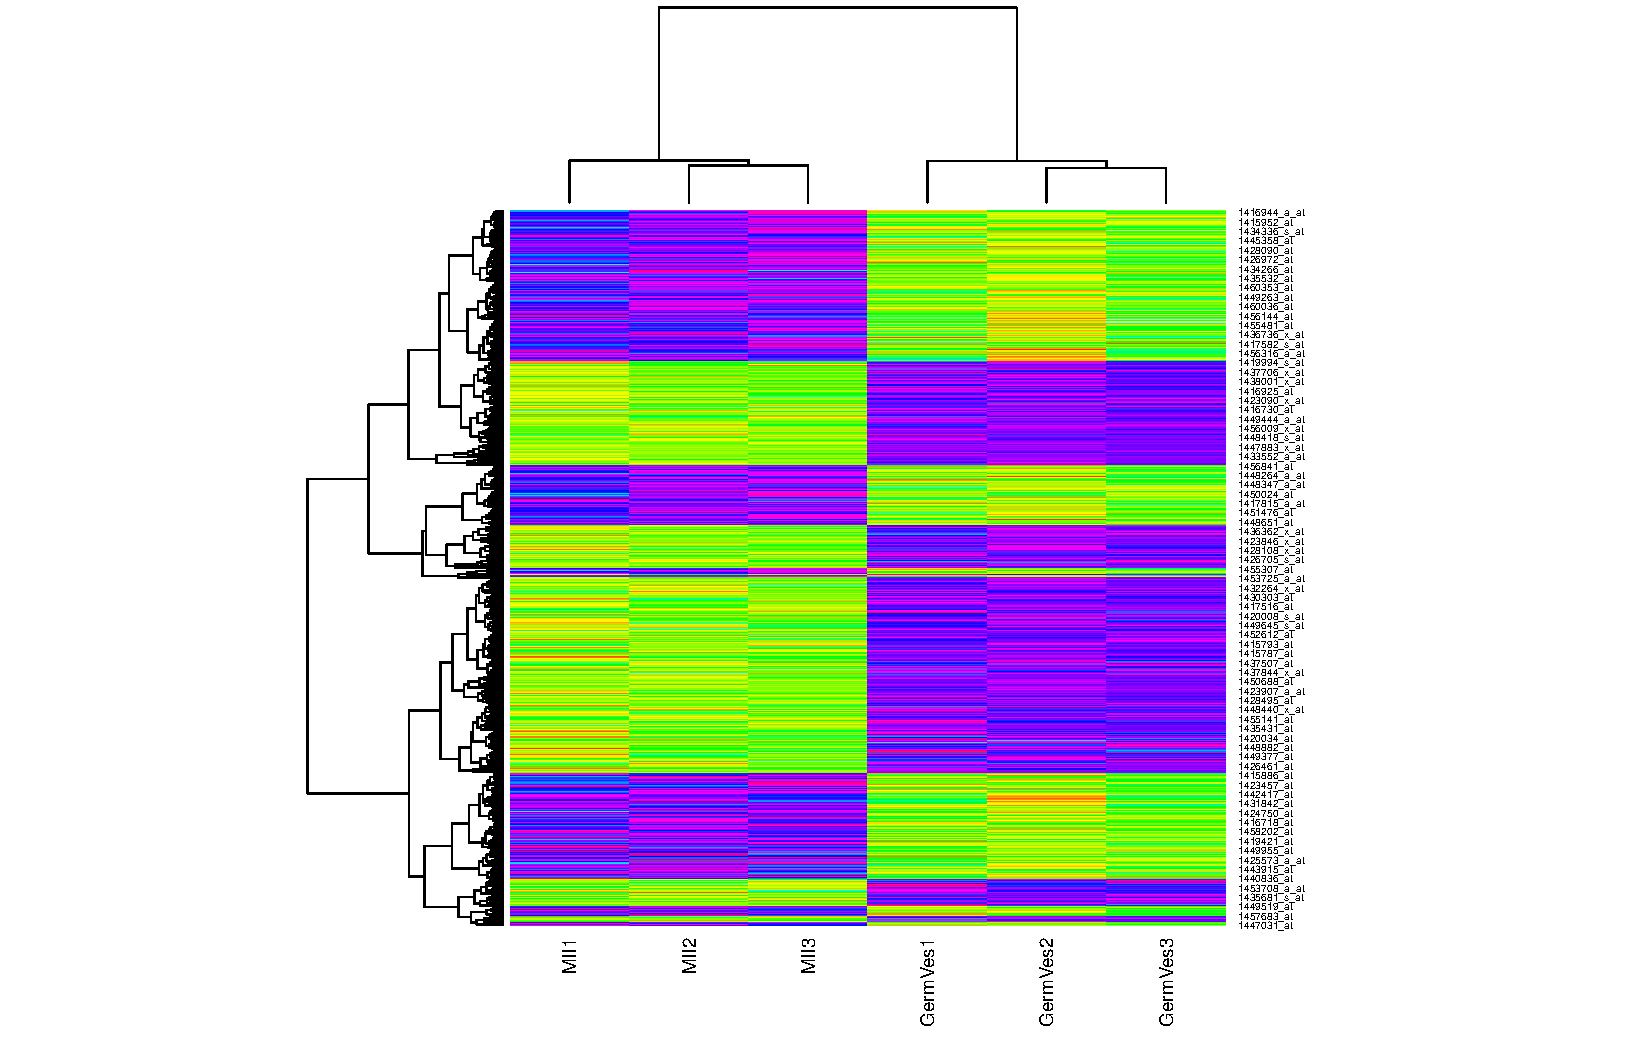
\includegraphics{Código-PEC1-Nuevo_files/figure-latex/unnamed-chunk-14-1.pdf}

\begin{Shaded}
\begin{Highlighting}[]
\OperatorTok{>}\StringTok{ }\KeywordTok{heatmap.2}\NormalTok{(exprs2cluster,}
\OperatorTok{+}\StringTok{           }\DataTypeTok{col =}\NormalTok{ bluered, }\DataTypeTok{scale =} \StringTok{"row"}\NormalTok{, }\DataTypeTok{key =} \OtherTok{TRUE}\NormalTok{, }\DataTypeTok{symkey =} \OtherTok{FALSE}\NormalTok{,}
\OperatorTok{+}\StringTok{           }\DataTypeTok{density.info =} \StringTok{"none"}\NormalTok{, }\DataTypeTok{trace =} \StringTok{"none"}\NormalTok{, }\DataTypeTok{cexCol =} \DecValTok{1}\NormalTok{, }\DataTypeTok{sepwidth =} \KeywordTok{c}\NormalTok{(}\FloatTok{0.05}\NormalTok{, }\FloatTok{0.05}\NormalTok{))}
\end{Highlighting}
\end{Shaded}

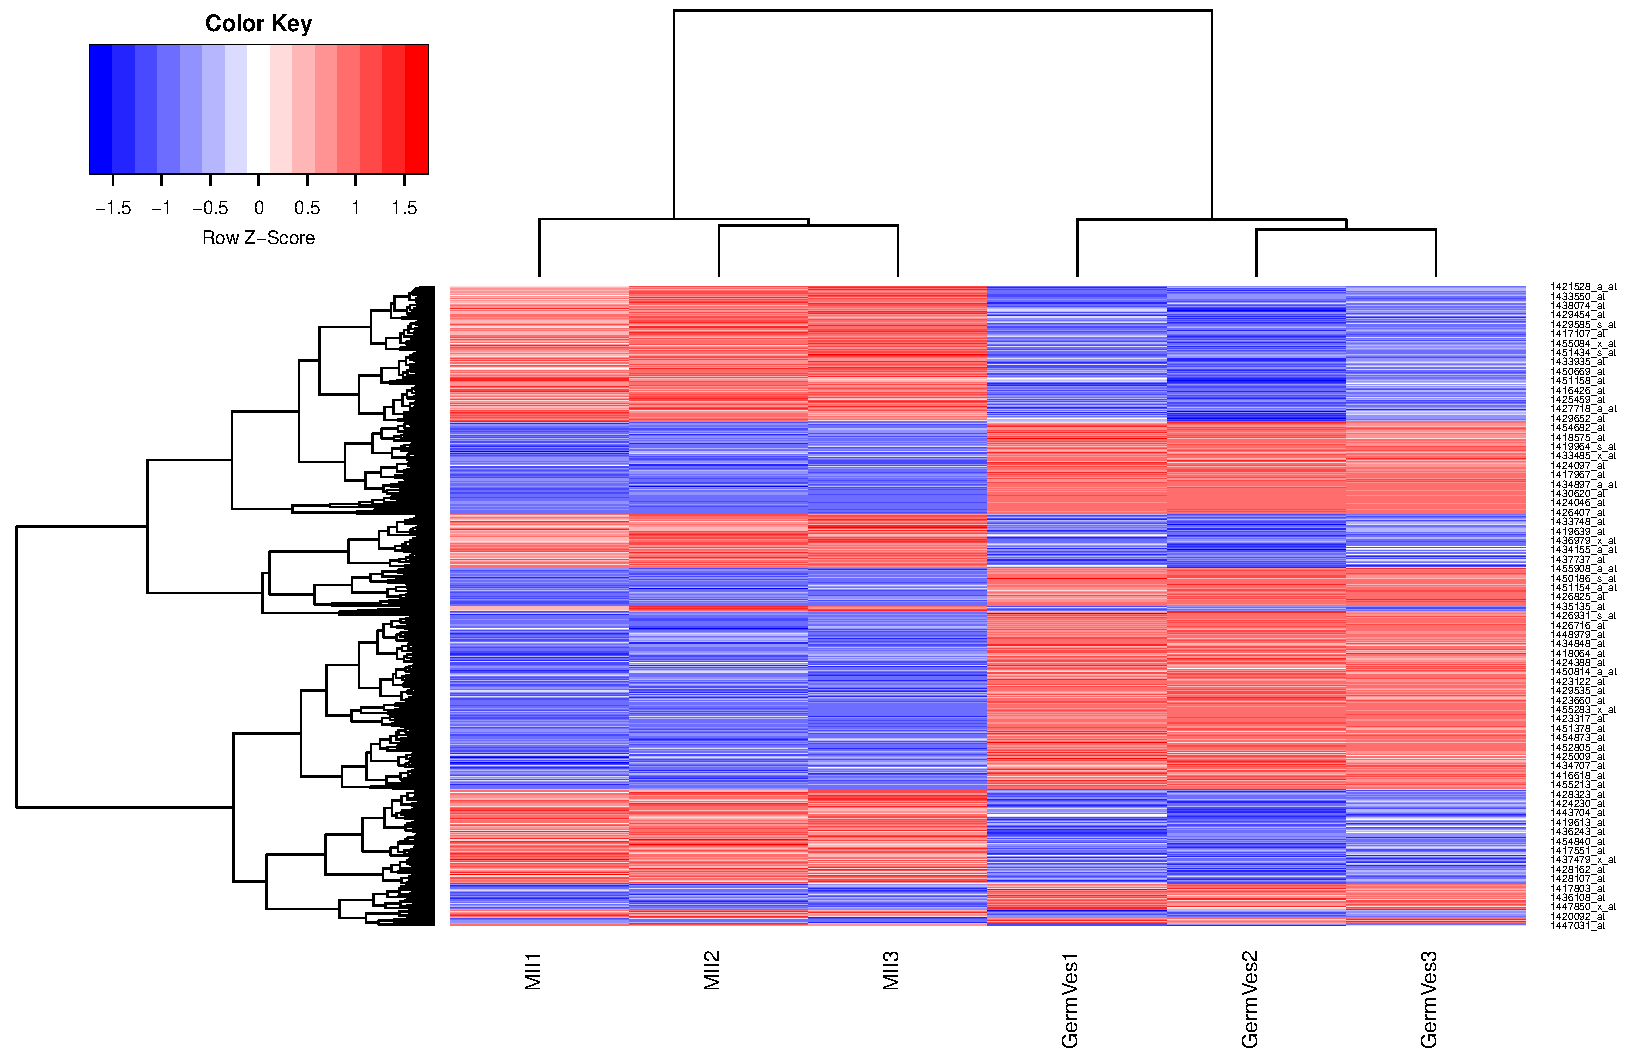
\includegraphics{Código-PEC1-Nuevo_files/figure-latex/unnamed-chunk-15-1.pdf}

\hypertarget{anuxe1lisis-de-la-significaciuxf3n-bioluxf3gica}{%
\subsection{Análisis de la significación
biológica}\label{anuxe1lisis-de-la-significaciuxf3n-bioluxf3gica}}

\hypertarget{go-set-enrichment-utilizando-la-ontologuxeda-biological-process.}{%
\subsubsection{GO Set Enrichment utilizando la ontología: Biological
Process.}\label{go-set-enrichment-utilizando-la-ontologuxeda-biological-process.}}

\begin{Shaded}
\begin{Highlighting}[]
\OperatorTok{>}\StringTok{ }\NormalTok{ego <-}\StringTok{ }\KeywordTok{enrichGO}\NormalTok{(gene, }\DataTypeTok{OrgDb =} \StringTok{"org.Mm.eg.db"}\NormalTok{, }\DataTypeTok{ont=}\StringTok{"BP"}\NormalTok{, }\DataTypeTok{readable=}\OtherTok{TRUE}\NormalTok{)}
\OperatorTok{>}\StringTok{ }\KeywordTok{barplot}\NormalTok{(ego, }\DataTypeTok{showCategory=}\DecValTok{25}\NormalTok{)}
\end{Highlighting}
\end{Shaded}

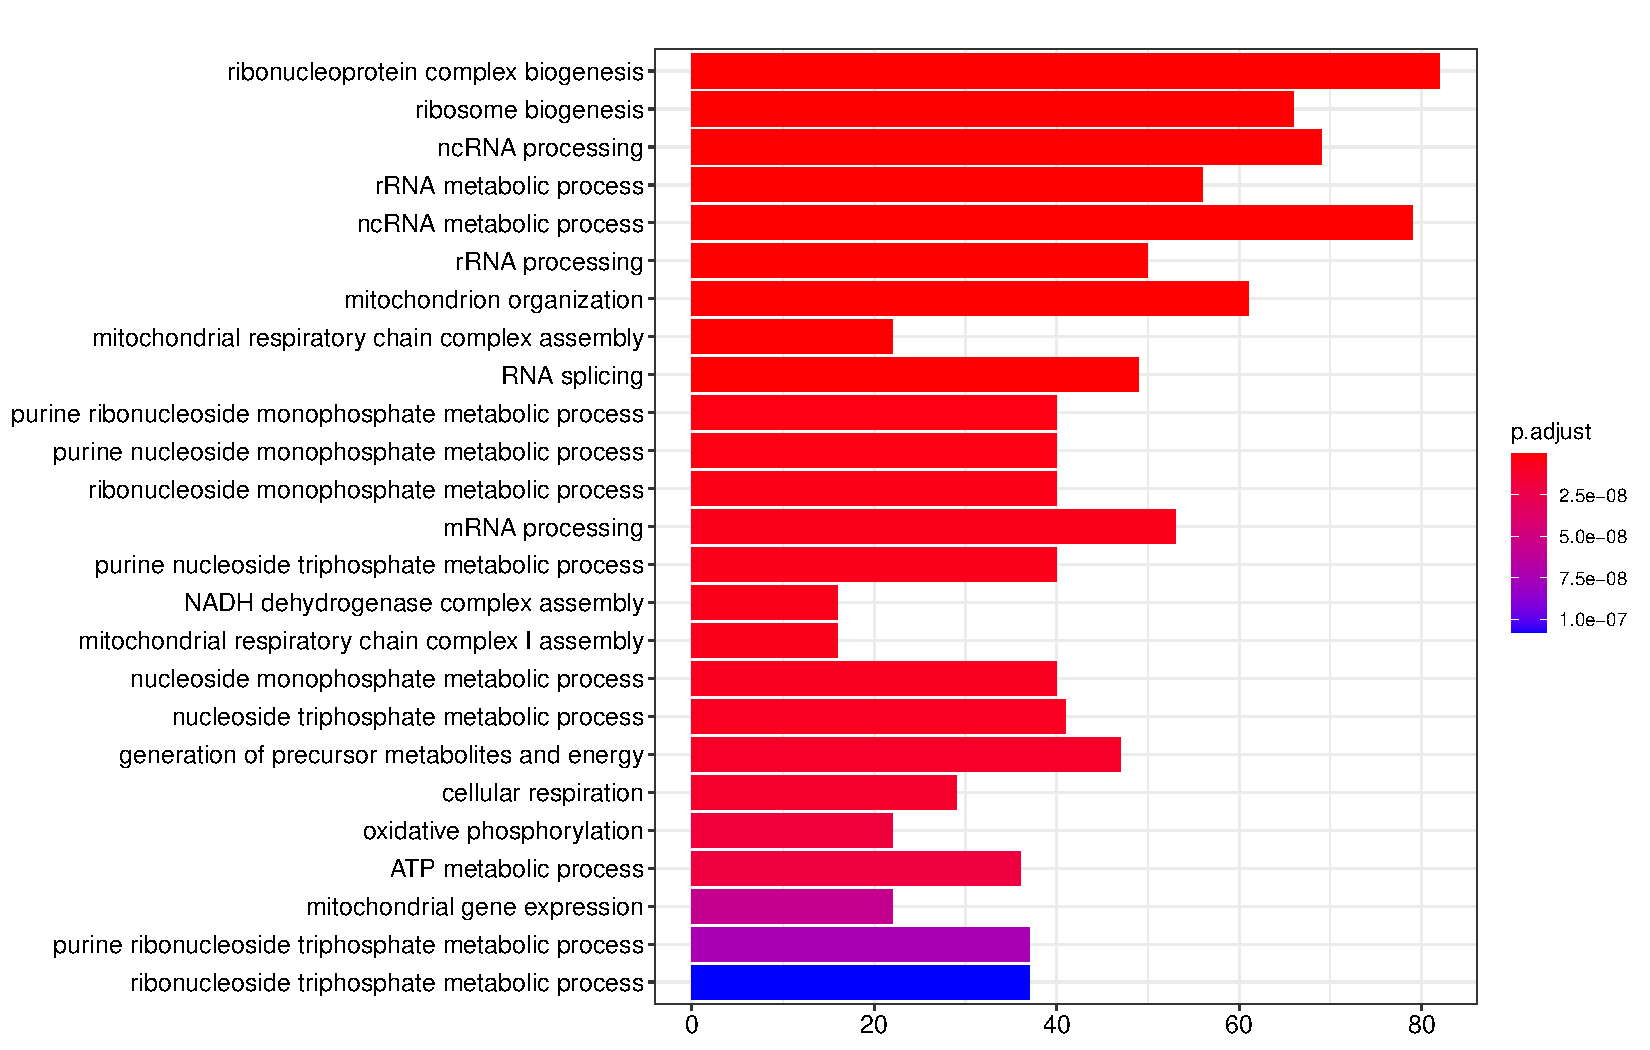
\includegraphics{Código-PEC1-Nuevo_files/figure-latex/unnamed-chunk-16-1.pdf}

\begin{Shaded}
\begin{Highlighting}[]
\OperatorTok{>}\StringTok{ }\KeywordTok{dotplot}\NormalTok{(ego, }\DataTypeTok{showCategory=}\DecValTok{30}\NormalTok{)}
\end{Highlighting}
\end{Shaded}

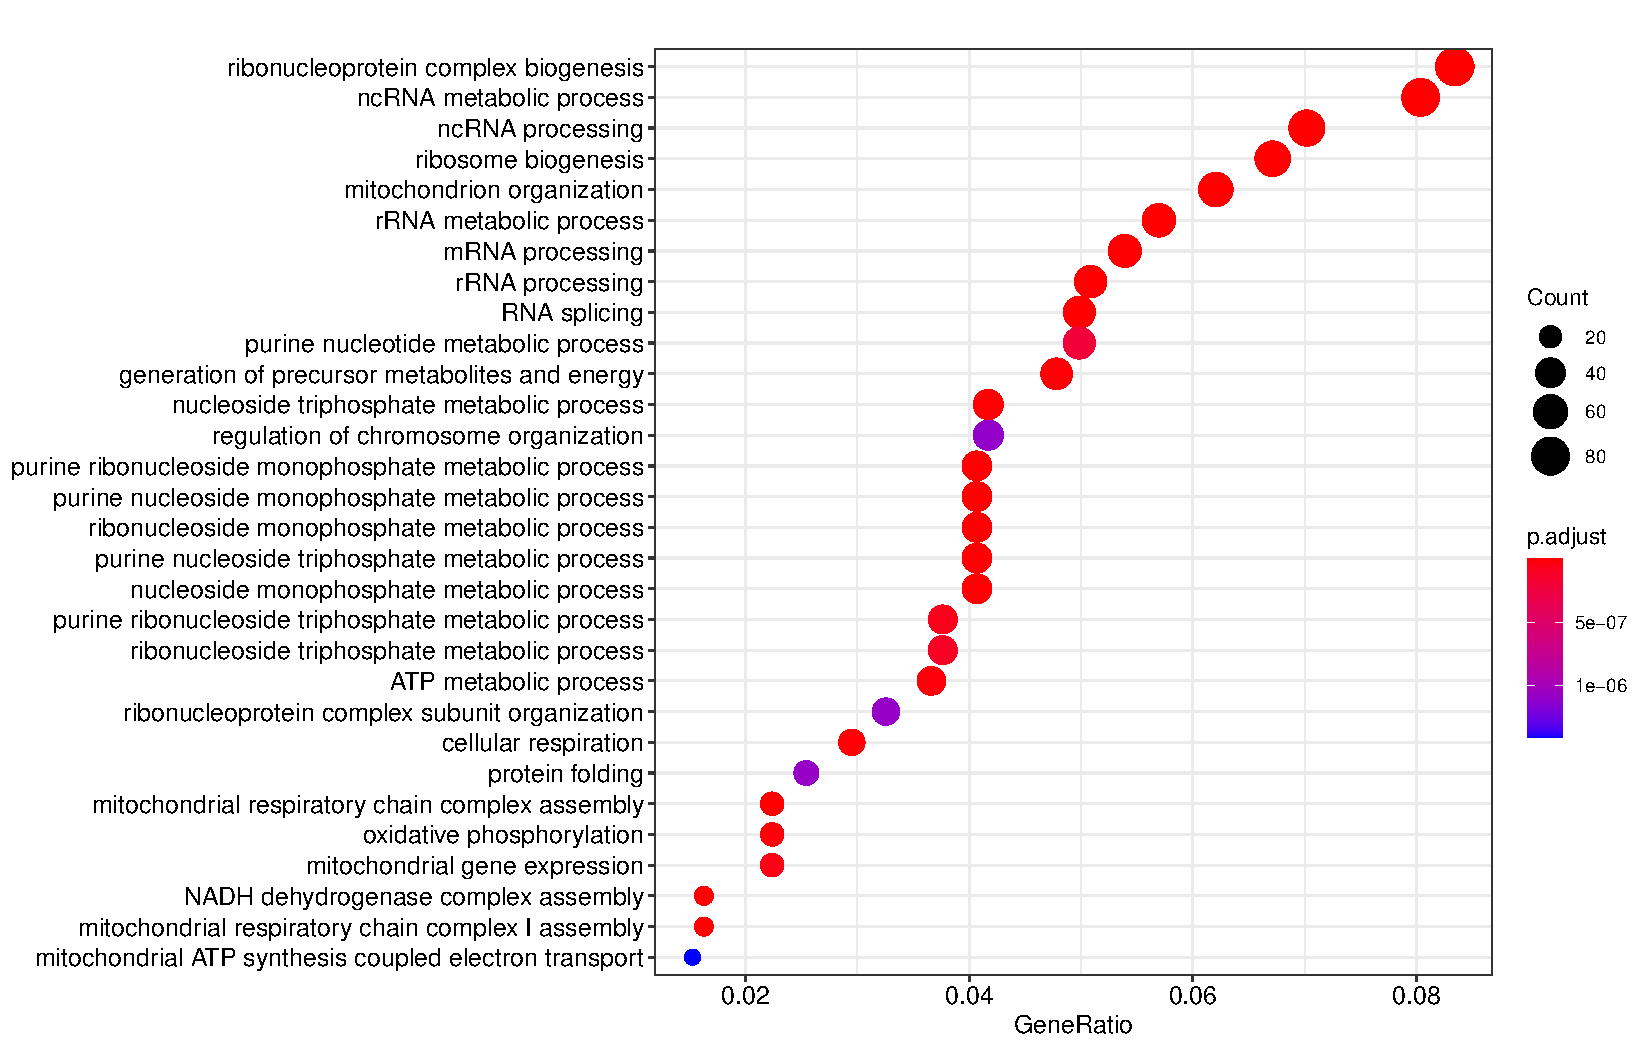
\includegraphics{Código-PEC1-Nuevo_files/figure-latex/unnamed-chunk-16-2.pdf}

\begin{Shaded}
\begin{Highlighting}[]
\OperatorTok{>}\StringTok{ }\NormalTok{go <-}\StringTok{ }\KeywordTok{enrichGO}\NormalTok{(gene, }\DataTypeTok{OrgDb =} \StringTok{"org.Mm.eg.db"}\NormalTok{, }\DataTypeTok{ont=}\StringTok{"all"}\NormalTok{)}
\OperatorTok{>}\StringTok{ }\KeywordTok{dotplot}\NormalTok{(go, }\DataTypeTok{split=}\StringTok{"ONTOLOGY"}\NormalTok{) }\OperatorTok{+}\StringTok{ }\KeywordTok{facet_grid}\NormalTok{(ONTOLOGY}\OperatorTok{~}\NormalTok{., }\DataTypeTok{scale=}\StringTok{"free"}\NormalTok{)}
\end{Highlighting}
\end{Shaded}

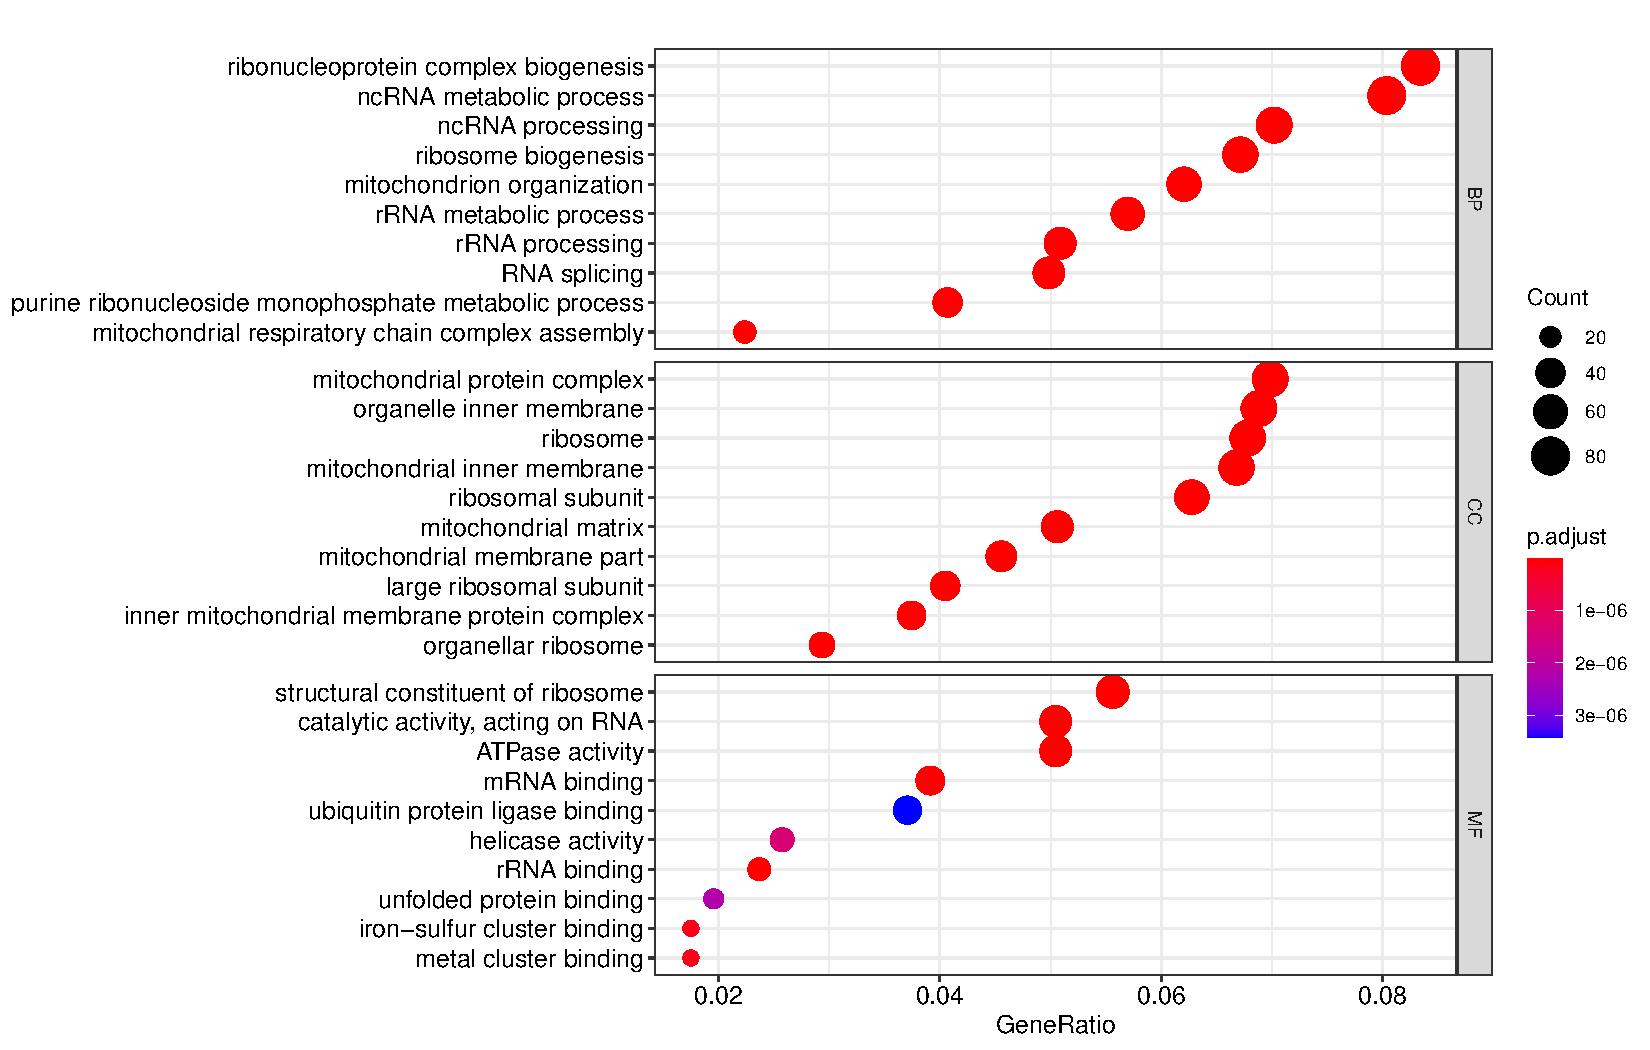
\includegraphics{Código-PEC1-Nuevo_files/figure-latex/unnamed-chunk-16-3.pdf}

\hypertarget{visualizaciuxf3n-de-cluxfasters-mediante-cnetplot}{%
\subsubsection{Visualización de clústers mediante
cnetplot}\label{visualizaciuxf3n-de-cluxfasters-mediante-cnetplot}}

\begin{Shaded}
\begin{Highlighting}[]
\OperatorTok{>}\StringTok{ }\NormalTok{ego2 <-}\StringTok{ }\KeywordTok{simplify}\NormalTok{(ego)}
\OperatorTok{>}\StringTok{ }\KeywordTok{cnetplot}\NormalTok{(ego2, }\DataTypeTok{foldChange=}\NormalTok{geneList)}
\end{Highlighting}
\end{Shaded}

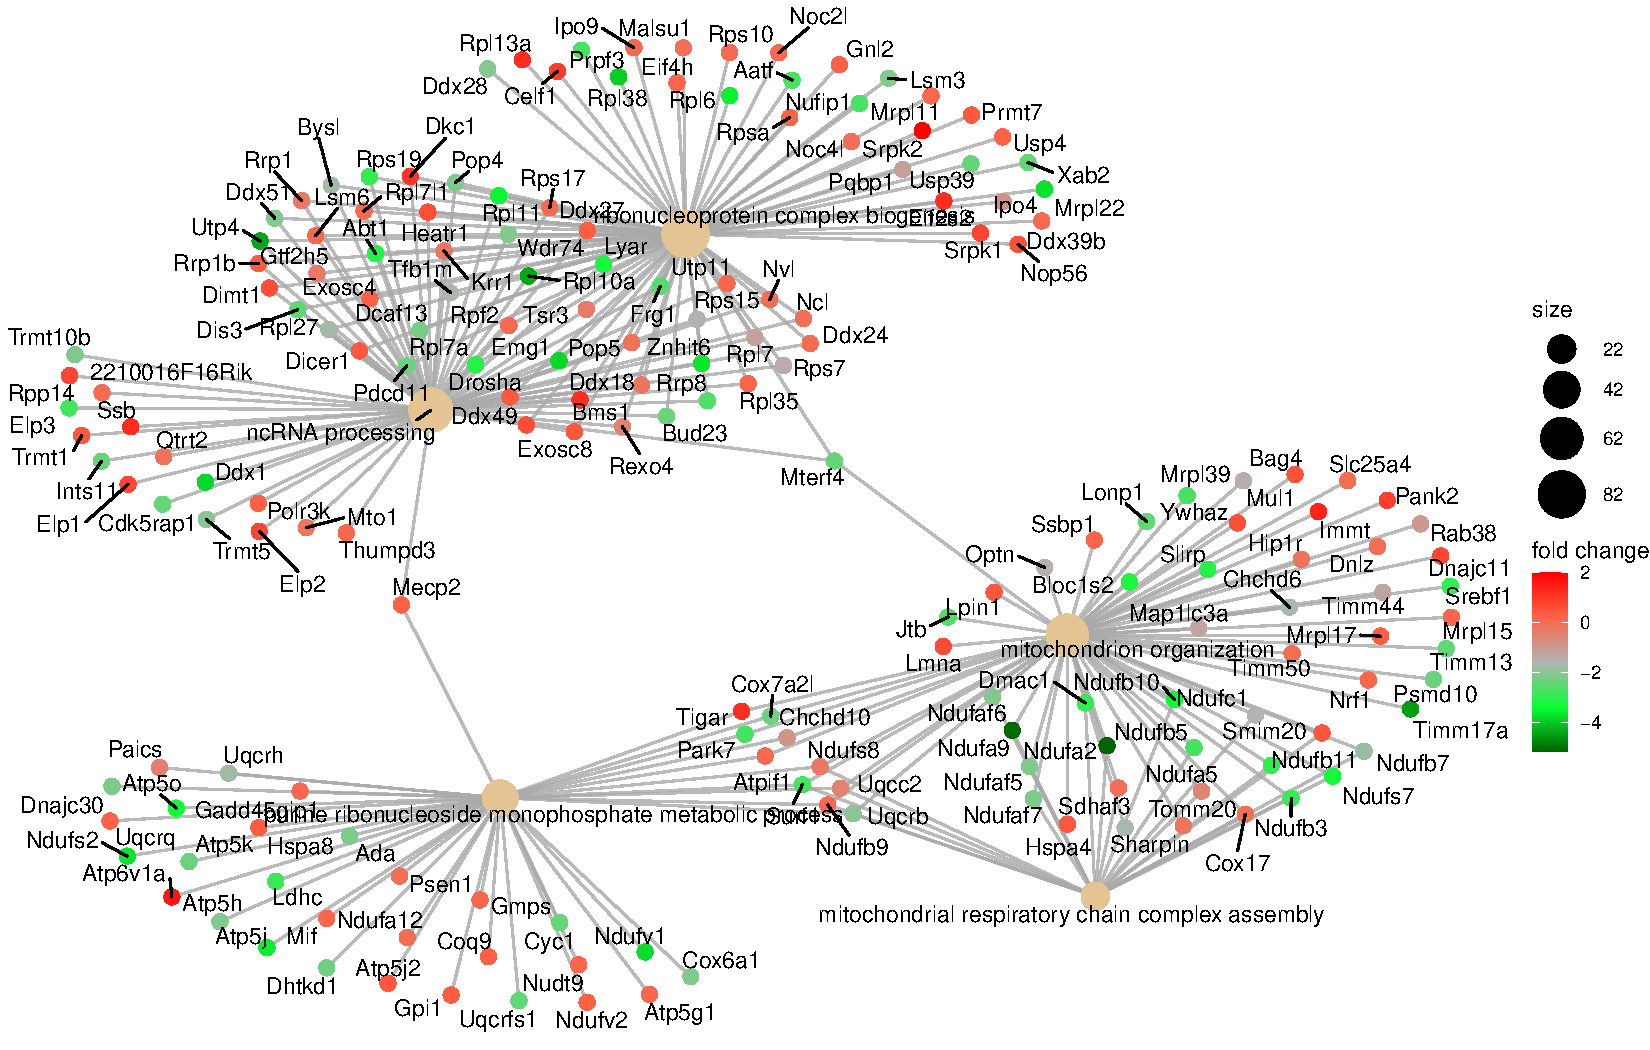
\includegraphics{Código-PEC1-Nuevo_files/figure-latex/unnamed-chunk-17-1.pdf}

\hypertarget{kegg-set-enrichment-using-clusterprofiler}{%
\subsubsection{KEGG set enrichment using
clusterProfiler}\label{kegg-set-enrichment-using-clusterprofiler}}

\begin{Shaded}
\begin{Highlighting}[]
\OperatorTok{>}\StringTok{ }\NormalTok{kk <-}\StringTok{ }\KeywordTok{enrichKEGG}\NormalTok{(}\DataTypeTok{gene =}\NormalTok{ gene, }\DataTypeTok{organism =} \StringTok{"mmu"}\NormalTok{, }\DataTypeTok{pvalueCutoff =} \FloatTok{0.05}\NormalTok{)}
\OperatorTok{>}\StringTok{ }\KeywordTok{head}\NormalTok{(kk)}
\end{Highlighting}
\end{Shaded}

\begin{verbatim}
               ID                               Description GeneRatio  BgRatio
mmu05012 mmu05012                         Parkinson disease    57/459 247/8775
mmu03010 mmu03010                                  Ribosome    42/459 175/8775
mmu00190 mmu00190                 Oxidative phosphorylation    36/459 133/8775
mmu05016 mmu05016                        Huntington disease    46/459 268/8775
mmu04932 mmu04932 Non-alcoholic fatty liver disease (NAFLD)    32/459 150/8775
mmu04714 mmu04714                             Thermogenesis    40/459 230/8775
               pvalue     p.adjust       qvalue
mmu05012 2.116513e-22 5.989732e-20 5.547492e-20
mmu03010 2.181157e-17 3.086337e-15 2.858463e-15
mmu00190 7.358811e-17 6.941812e-15 6.429277e-15
mmu05016 4.449123e-13 3.147754e-11 2.915346e-11
mmu04932 5.118315e-12 2.896967e-10 2.683075e-10
mmu04714 1.068575e-11 5.040113e-10 4.667987e-10
                                                                                                                                                                                                                                                                                                                                                            geneID
mmu05012 22145/66108/59029/72900/17991/69077/17995/73710/19173/19170/14828/28080/75406/22190/19181/66997/71679/226646/104130/66576/20463/11957/22154/57320/66218/66413/68015/22335/23996/19175/19172/67680/67128/26408/68342/225887/66495/11951/11739/66594/68202/66694/26443/56436/19167/66414/66916/22272/227613/12861/67530/18803/66046/11911/66445/19182/66377
mmu03010                                                                                             19896/20068/66489/67427/20115/27050/19899/67671/20084/67025/19989/27397/68735/66258/19942/22121/216767/26451/19988/16785/68028/67097/76808/20090/76846/56282/27370/121022/27207/67281/14109/26961/19981/27176/66419/19921/94063/20054/20085/94064/27395/68611
mmu00190                                                                                                                                66108/11984/72900/17991/17995/28080/57423/75406/71679/226646/104130/66576/20463/11957/73834/66218/11973/11964/67680/12856/68342/225887/66495/11951/66594/68202/11958/66694/66414/66916/22272/12861/67530/66046/66445/66377
mmu05016                                                                  231329/22145/66108/72900/17991/17995/73710/28080/75406/71679/18181/226646/104130/66576/20463/11957/22154/66218/22335/26400/67680/26408/68342/225887/66495/11951/13417/11739/66594/68202/66694/66414/66916/22272/227613/74325/12861/67530/69920/12757/66046/14682/66445/66377/69654/12914
mmu04932                                                                                                                                                        66108/72900/17991/17995/20787/75406/226646/104130/66576/20463/18706/66218/67680/26408/68342/225887/66495/66594/68202/66694/66414/66916/22272/12702/12861/67530/66046/72674/11911/66445/66377/18708
mmu04714                                                                                                        66108/72900/17991/17995/28080/57423/75406/71679/226646/104130/66576/20463/11957/57376/66218/14784/67680/15461/26408/12856/68342/225887/66495/11951/66594/68202/11958/66694/66414/66916/22272/73694/12861/67530/66046/66445/66377/76947/70127/69487
         Count
mmu05012    57
mmu03010    42
mmu00190    36
mmu05016    46
mmu04932    32
mmu04714    40
\end{verbatim}

\begin{Shaded}
\begin{Highlighting}[]
\OperatorTok{>}\StringTok{ }\NormalTok{kk2 <-}\StringTok{ }\KeywordTok{gseKEGG}\NormalTok{(}\DataTypeTok{geneList =}\NormalTok{ geneList,}\DataTypeTok{organism =} \StringTok{"mmu"}\NormalTok{, }\DataTypeTok{nPerm =} \DecValTok{1000}\NormalTok{, }
\OperatorTok{+}\StringTok{                }\DataTypeTok{minGSSize =} \DecValTok{120}\NormalTok{, }\DataTypeTok{pvalueCutoff =} \FloatTok{0.05}\NormalTok{) }
\OperatorTok{>}\StringTok{ }\KeywordTok{head}\NormalTok{(kk2)}
\end{Highlighting}
\end{Shaded}

\begin{verbatim}
               ID                    Description setSize enrichmentScore
mmu05012 mmu05012              Parkinson disease     218      -0.5257865
mmu04714 mmu04714                  Thermogenesis     209      -0.4898015
mmu04071 mmu04071 Sphingolipid signaling pathway     120       0.5658919
mmu04611 mmu04611            Platelet activation     120       0.5241317
mmu05135 mmu05135             Yersinia infection     121       0.6000976
mmu04110 mmu04110                     Cell cycle     123       0.4630431
               NES      pvalue   p.adjust     qvalues rank
mmu05012 -1.615448 0.001067236 0.01715856 0.001407401 4016
mmu04714 -1.503035 0.004296455 0.01715856 0.001407401 5287
mmu04071  2.141527 0.006993007 0.01715856 0.001407401 6174
mmu04611  1.983492 0.006993007 0.01715856 0.001407401 7874
mmu05135  2.265665 0.007042254 0.01715856 0.001407401 8126
mmu04110  1.748651 0.007142857 0.01715856 0.001407401 5433
                           leading_edge
mmu05012  tags=30%, list=9%, signal=28%
mmu04714 tags=32%, list=12%, signal=28%
mmu04071 tags=28%, list=14%, signal=24%
mmu04611 tags=30%, list=17%, signal=25%
mmu05135 tags=29%, list=18%, signal=24%
mmu04110 tags=25%, list=12%, signal=22%
                                                                                                                                                                                                                                                                                                                                                                                                                                                                                                                                                                                                                                                                                                                                                                                                                                                                                                                                          core_enrichment
mmu05012 67089/13665/12858/12367/227613/227197/17993/22151/54405/26442/230075/12858/22142/11946/13063/26442/19170/16593/230075/19185/12859/12859/12857/66043/227613/68943/110323/228033/11911/26444/26444/66091/12859/225887/66416/66925/170731/66091/67942/11950/12859/17993/13063/14683/66377/105675/12325/56436/57296/13198/22151/66414/66576/20422/66416/66916/22186/67126/68349/20422/225887/67530/22190/78330/11911/11739/12861/56436/71679/66414/22145/19167/225887/19175/66414/11739/66594/66218/66218/225887/20463/20463/66576/68202/66445/23996/66377/26408/66694/22190/227613/22335/14828/20463/26443/67530/68015/11951/68015/66046/57320/11739/22190/19182/26443/18803/67680/66495/23996/225887/22190/66916/22154/71679/22190/66997/104130/66413/66046/67128/66413/19173/22272/75406/72900/57320/28080/68342/14828/104130/11957/104130/226646/19170/17995/73710/28080/69077/72900/19172/66108/75406/19181/17991/22145/17995/59029/19181/17995
mmu04714                                  68493/66152/50721/66052/67130/68202/68198/12862/110323/12913/66416/67184/11949/11515/20587/66416/67264/76178/12896/67892/20587/50790/216739/20111/14081/66272/12858/83796/227197/17993/12913/19092/64930/20662/57279/54405/12913/230075/12858/11946/70383/230075/12859/70673/12859/20586/12857/66043/110323/228033/20104/56456/66091/12859/19082/225887/66416/66925/66091/56456/67942/11950/12859/17993/68094/68033/14683/12896/83379/66377/69893/27425/11465/19082/57279/67155/15461/66414/66576/66416/66916/67126/68349/225887/67530/78330/76947/12861/71679/69487/66414/225887/73694/66414/66594/66218/66218/225887/20463/20463/66576/11958/68202/66445/70127/66377/26408/66694/20463/11958/67530/11951/66046/12856/14784/15461/67680/66495/225887/11958/66916/71679/104130/66046/22272/75406/57423/72900/28080/68342/57376/104130/11957/104130/226646/17995/57423/28080/72900/66108/75406/17991/17995/17995
mmu04071                                                                                                                                                                                                                                                                                                                                                                                                                  26416/54447/14678/26408/110157/18798/19877/14673/14674/14677/26420/14674/26931/14674/19877/23797/619326/18607/14682/26417/11651/18176/26416/11651/26415/18708/26931/26396/14673/14673/23797/26931/22059/26416/71978/26413/110157/11652/268656/18708/26932/26419/433323/18805/23797/51792/110157/18805/18706/26420/18797/22059/26932/170758/18751/19353/26395/26419/14360/19697/18607/18805/26419/26931/26932/19052/73699/268656/18706/18754/13244/14682/14677/12122/18754/18762/19211/18750/18033/26931/51792/14673/51792/51792
mmu04611                                                                                                                                                                                                                                                                                                                                                                                                                       19046/26416/14678/19045/69632/18798/19877/14674/14677/14674/18747/17931/14674/19877/23797/14682/232906/11515/26417/19092/11651/26416/12229/21894/11651/26415/18708/23797/19047/26416/232889/26413/11652/11461/18708/16439/19047/20619/23797/19091/18749/16438/17931/18747/215449/18706/19046/18797/16439/11461/67268/19046/14360/11461/67268/18706/14682/18759/14677/109905/108101/16822/18762/19092/11461/16440/19046/210044/67938/228785/215449/19395/60596/234889/14683/14677/11514/20963/11651/18795/20866/19094/18798
mmu05135                                                                                                                                                                                                                                                                                                                                         26416/69632/19877/68652/26420/26398/18035/19877/23797/11845/26417/12540/18035/11651/12928/14083/26416/16179/11651/26415/18708/19303/26396/19303/14083/23797/242687/20112/26416/12929/54126/26413/11652/11461/18708/330662/26419/73178/18019/18719/26409/23797/54353/68652/18706/26420/26398/170758/11461/19353/26395/26419/18719/109333/17874/19697/26419/11461/18706/11845/12928/16402/108100/18019/67071/16179/16822/26409/22034/18717/11461/22034/18033/12928/16402/68524/56637/73178/22034/56637/56480/66513/18018/108100/16818/16885/11651/330319/19229/19094/83564/16797/16179/110651/12929/110596
mmu04110                                                                                                                                                                                                                                                                                                                                                                                                                                                     69957/21402/52563/66440/22627/56637/381759/22627/18393/12580/22627/229776/12444/22629/433759/17215/18393/17873/12237/217232/22631/12444/245000/17215/12237/52206/17219/17128/17215/17219/17126/52206/12531/21809/22642/211586/26428/12534/12444/12235/12576/12572/140557/12443/12649/12566/24061/12448/22630/21808/56371/242705/26428/54401/19090/19650/22630/22390/12444/12572/12530/22631/22137/12532/22630/17218/22630/99152/12444/12532/22630/66671/12444/211586/12235/23834/56317/66671
\end{verbatim}

\begin{Shaded}
\begin{Highlighting}[]
\OperatorTok{>}\StringTok{ }\KeywordTok{dotplot}\NormalTok{(kk, }\DataTypeTok{showCategory=}\DecValTok{20}\NormalTok{)}
\end{Highlighting}
\end{Shaded}

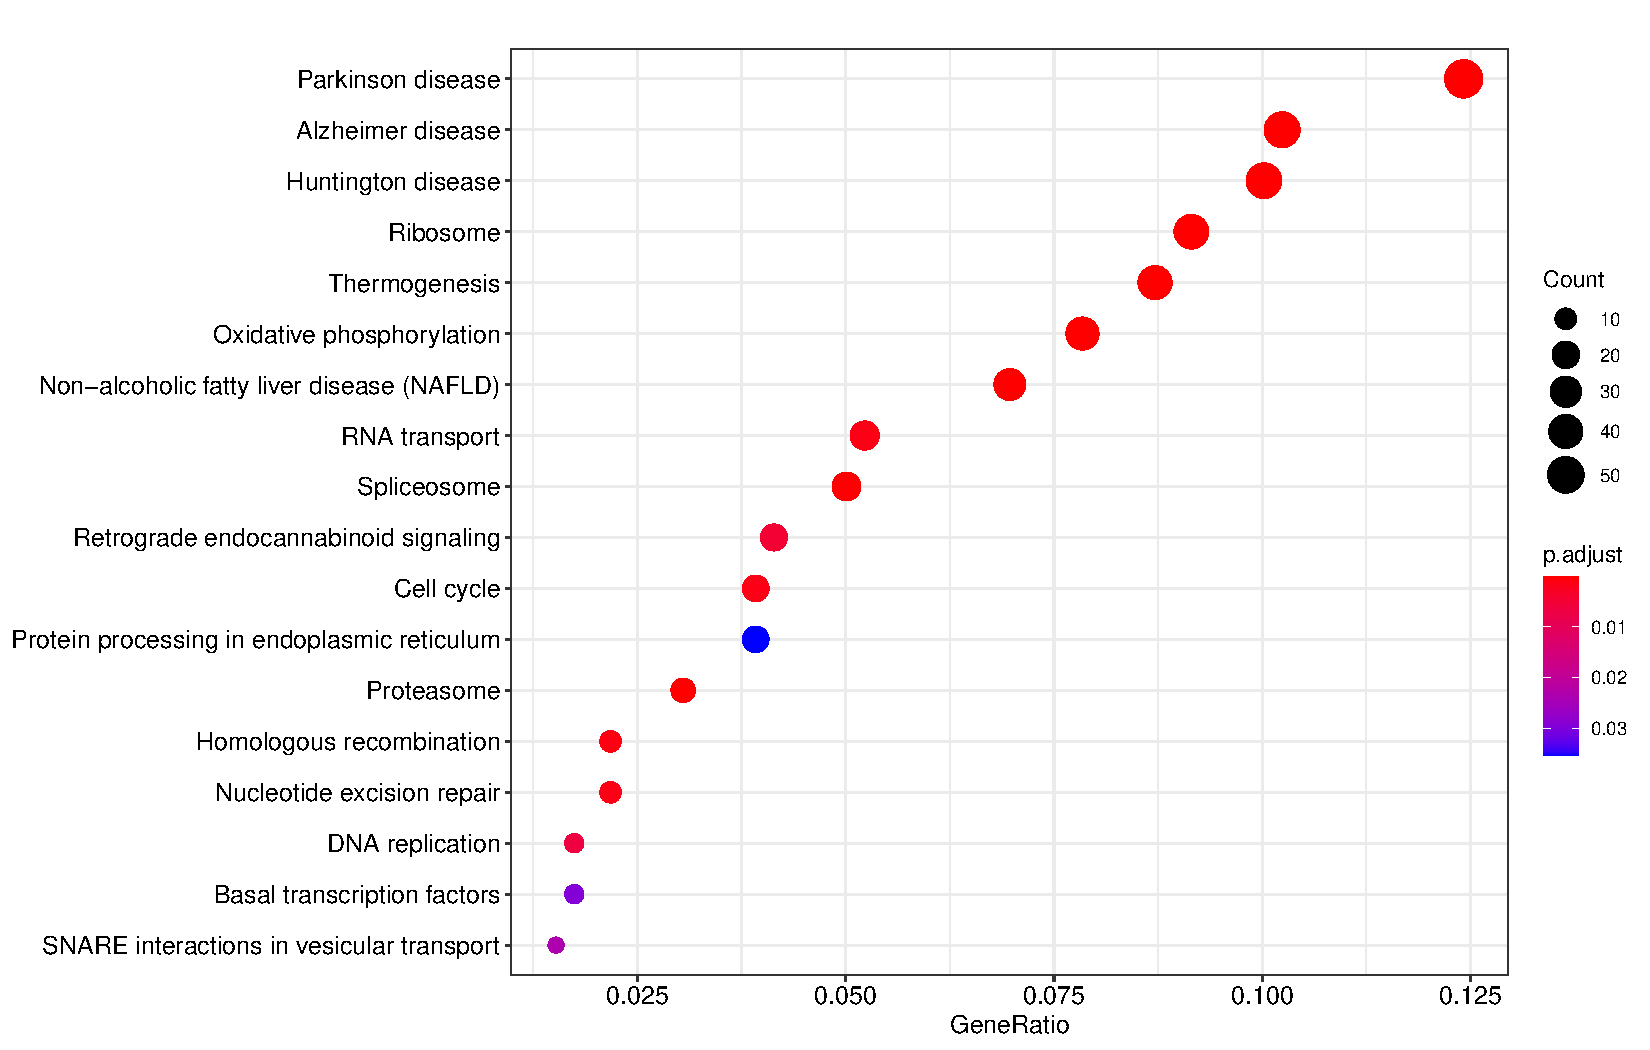
\includegraphics{Código-PEC1-Nuevo_files/figure-latex/unnamed-chunk-18-1.pdf}

\begin{Shaded}
\begin{Highlighting}[]
\OperatorTok{>}\StringTok{ }\NormalTok{wnt <-}\StringTok{ }\KeywordTok{pathview}\NormalTok{(}\DataTypeTok{gene.data =}\NormalTok{ geneList,}
\OperatorTok{+}\StringTok{                 }\DataTypeTok{pathway.id =} \StringTok{"mmu04310"}\NormalTok{,}
\OperatorTok{+}\StringTok{                 }\DataTypeTok{species =} \StringTok{"mmu"}\NormalTok{,}
\OperatorTok{+}\StringTok{                 }\DataTypeTok{limit =} \KeywordTok{list}\NormalTok{(}\DataTypeTok{gene=}\KeywordTok{max}\NormalTok{(}\KeywordTok{abs}\NormalTok{(geneList)), }\DataTypeTok{cpd=}\DecValTok{1}\NormalTok{))}
\OperatorTok{>}\StringTok{ }
\ErrorTok{>}\StringTok{ }\NormalTok{ampk <-}\StringTok{ }\KeywordTok{pathview}\NormalTok{(}\DataTypeTok{gene.data =}\NormalTok{ geneList,}
\OperatorTok{+}\StringTok{                  }\DataTypeTok{pathway.id =} \StringTok{"mmu04152"}\NormalTok{,}
\OperatorTok{+}\StringTok{                  }\DataTypeTok{species =} \StringTok{"mmu"}\NormalTok{,}
\OperatorTok{+}\StringTok{                  }\DataTypeTok{limit =} \KeywordTok{list}\NormalTok{(}\DataTypeTok{gene=}\KeywordTok{max}\NormalTok{(}\KeywordTok{abs}\NormalTok{(geneList)), }\DataTypeTok{cpd=}\DecValTok{1}\NormalTok{))}
\OperatorTok{>}\StringTok{ }
\ErrorTok{>}\StringTok{ }\NormalTok{pi3pakt <-}\StringTok{ }\KeywordTok{pathview}\NormalTok{(}\DataTypeTok{gene.data =}\NormalTok{ geneList,}
\OperatorTok{+}\StringTok{                     }\DataTypeTok{pathway.id =} \StringTok{"mmu04151"}\NormalTok{,}
\OperatorTok{+}\StringTok{                     }\DataTypeTok{species =} \StringTok{"mmu"}\NormalTok{,}
\OperatorTok{+}\StringTok{                     }\DataTypeTok{limit =} \KeywordTok{list}\NormalTok{(}\DataTypeTok{gene=}\KeywordTok{max}\NormalTok{(}\KeywordTok{abs}\NormalTok{(geneList)), }\DataTypeTok{cpd=}\DecValTok{1}\NormalTok{))}
\OperatorTok{>}\StringTok{ }
\ErrorTok{>}\StringTok{ }\NormalTok{mapkinasa <-}\StringTok{ }\KeywordTok{pathview}\NormalTok{(}\DataTypeTok{gene.data =}\NormalTok{ geneList,}
\OperatorTok{+}\StringTok{                       }\DataTypeTok{pathway.id =} \StringTok{"mmu04010"}\NormalTok{,}
\OperatorTok{+}\StringTok{                       }\DataTypeTok{species =} \StringTok{"mmu"}\NormalTok{,}
\OperatorTok{+}\StringTok{                       }\DataTypeTok{limit =} \KeywordTok{list}\NormalTok{(}\DataTypeTok{gene=}\KeywordTok{max}\NormalTok{(}\KeywordTok{abs}\NormalTok{(geneList)), }\DataTypeTok{cpd=}\DecValTok{1}\NormalTok{))}
\OperatorTok{>}\StringTok{ }
\ErrorTok{>}\StringTok{ }\NormalTok{oxpho <-}\StringTok{ }\KeywordTok{pathview}\NormalTok{(}\DataTypeTok{gene.data =}\NormalTok{ geneList,}
\OperatorTok{+}\StringTok{                   }\DataTypeTok{pathway.id =} \StringTok{"mmu00190"}\NormalTok{,}
\OperatorTok{+}\StringTok{                   }\DataTypeTok{species =} \StringTok{"mmu"}\NormalTok{,}
\OperatorTok{+}\StringTok{                   }\DataTypeTok{limit =} \KeywordTok{list}\NormalTok{(}\DataTypeTok{gene=}\KeywordTok{max}\NormalTok{(}\KeywordTok{abs}\NormalTok{(geneList)), }\DataTypeTok{cpd=}\DecValTok{1}\NormalTok{))}
\OperatorTok{>}\StringTok{ }
\ErrorTok{>}\StringTok{ }\NormalTok{ribo <-}\StringTok{ }\KeywordTok{pathview}\NormalTok{(}\DataTypeTok{gene.data =}\NormalTok{ geneList,}
\OperatorTok{+}\StringTok{                  }\DataTypeTok{pathway.id =} \StringTok{"mmu03010"}\NormalTok{,}
\OperatorTok{+}\StringTok{                  }\DataTypeTok{species =} \StringTok{"mmu"}\NormalTok{,}
\OperatorTok{+}\StringTok{                  }\DataTypeTok{limit =} \KeywordTok{list}\NormalTok{(}\DataTypeTok{gene=}\KeywordTok{max}\NormalTok{(}\KeywordTok{abs}\NormalTok{(geneList)), }\DataTypeTok{cpd=}\DecValTok{1}\NormalTok{))}
\end{Highlighting}
\end{Shaded}

\hypertarget{segundo-enfoque-de-gokegg}{%
\subsubsection{Segundo enfoque de
GO/KEGG}\label{segundo-enfoque-de-gokegg}}

Realizaremos un segundo GO /KEGG set enrichment y compararemos los
resultados. Seleccionaremos genes y pathways que hayan sido detectado en
ambos análisis.

El objeto ``dat.s'' contiene solo los genes diferencialmente expresados.
A partir de ahí se trabajará con el objeto ``myids'', que consta de
todos los probes que hemos considerado interesantes para el estudio. El
test que llevaremos a cabo ahora consiste en 3 pasos, ya que la
jerarquía de Gene Ontology (GO) consiste en tres diferentes ontologías:
procesos biológicos (BP), función molecular (MF) y componente celular
(CC).Estos comandos utilizan el pvalor de 0.05 para realizar el análisis
de los datos.

\begin{Shaded}
\begin{Highlighting}[]
\OperatorTok{>}\StringTok{ }\NormalTok{rn <-}\StringTok{ }\KeywordTok{rownames}\NormalTok{(}\KeywordTok{topTable}\NormalTok{(fit.main, }\DataTypeTok{n=}\DecValTok{100}\NormalTok{))}
\OperatorTok{>}\StringTok{ }\NormalTok{tt <-}\StringTok{ }\KeywordTok{topTable}\NormalTok{(fit.main, }\DataTypeTok{n=}\KeywordTok{nrow}\NormalTok{(ovo.rma))}
\OperatorTok{>}\StringTok{ }\NormalTok{rn <-}\StringTok{ }\KeywordTok{rownames}\NormalTok{(tt)[tt}\OperatorTok{$}\NormalTok{P.Value}\OperatorTok{<=}\FloatTok{0.001}\NormalTok{]}
\OperatorTok{>}\StringTok{ }\NormalTok{dat.s <-}\StringTok{ }\NormalTok{ovo.rma[rn,]}
\OperatorTok{>}\StringTok{ }\KeywordTok{head}\NormalTok{(dat.s)}
\end{Highlighting}
\end{Shaded}

\begin{verbatim}
             GermVes1 GermVes2 GermVes3     MII1     MII2     MII3
1433984_a_at 10.26365 10.15436 10.17803 3.853348 3.937798 3.981797
1456012_x_at 12.01688 12.08720 12.15211 5.981015 5.970370 5.808870
1438179_s_at 13.19012 13.16334 13.13278 7.811837 7.718080 7.832707
1437510_x_at 11.47459 11.74125 11.52850 4.680788 4.907036 4.580200
1429627_at   10.24633 10.40971 10.19094 3.891292 3.970757 3.633696
1433552_a_at 11.27960 11.45303 11.29181 5.567078 5.759502 5.448151
\end{verbatim}

\begin{Shaded}
\begin{Highlighting}[]
\OperatorTok{>}\StringTok{ }\NormalTok{aallg <-}\StringTok{ }\KeywordTok{get}\NormalTok{(}\StringTok{"mouse4302ENTREZID"}\NormalTok{)}
\OperatorTok{>}\StringTok{ }\NormalTok{allg <-}\StringTok{ }\KeywordTok{as.data.frame}\NormalTok{(}\KeywordTok{unlist}\NormalTok{(}\KeywordTok{as.list}\NormalTok{(aallg)))}
\OperatorTok{>}\StringTok{ }\NormalTok{myids <-}\StringTok{ }\KeywordTok{unique}\NormalTok{(allg[}\KeywordTok{rownames}\NormalTok{(dat.s),])}
\end{Highlighting}
\end{Shaded}

\begin{Shaded}
\begin{Highlighting}[]
\OperatorTok{>}\StringTok{ }\NormalTok{paramsBP <-}\StringTok{ }\KeywordTok{new}\NormalTok{(}\StringTok{"GOHyperGParams"}\NormalTok{, }\DataTypeTok{geneIds =}\NormalTok{ myids,}
\OperatorTok{+}\StringTok{                 }\DataTypeTok{annotation =} \KeywordTok{c}\NormalTok{(}\StringTok{"mouse4302.db"}\NormalTok{), }\DataTypeTok{ontology =} \StringTok{"BP"}\NormalTok{, }\DataTypeTok{pvalueCutoff =} \FloatTok{0.05}\NormalTok{,}
\OperatorTok{+}\StringTok{                 }\DataTypeTok{conditional =} \OtherTok{FALSE}\NormalTok{, }\DataTypeTok{testDirection =} \StringTok{"over"}\NormalTok{)}
\OperatorTok{>}\StringTok{ }\NormalTok{resultBP <-}\StringTok{ }\KeywordTok{hyperGTest}\NormalTok{(paramsBP)}
\OperatorTok{>}\StringTok{ }\NormalTok{paramsMF <-}\StringTok{ }\KeywordTok{new}\NormalTok{(}\StringTok{"GOHyperGParams"}\NormalTok{, }\DataTypeTok{geneIds =}\NormalTok{ myids,}
\OperatorTok{+}\StringTok{                 }\DataTypeTok{annotation =} \KeywordTok{c}\NormalTok{(}\StringTok{"mouse4302.db"}\NormalTok{), }\DataTypeTok{ontology =} \StringTok{"MF"}\NormalTok{, }\DataTypeTok{pvalueCutoff =} \FloatTok{0.05}\NormalTok{,}
\OperatorTok{+}\StringTok{                 }\DataTypeTok{conditional =} \OtherTok{FALSE}\NormalTok{, }\DataTypeTok{testDirection =} \StringTok{"over"}\NormalTok{)}
\OperatorTok{>}\StringTok{ }\NormalTok{resultMF <-}\StringTok{ }\KeywordTok{hyperGTest}\NormalTok{(paramsMF)}
\OperatorTok{>}\StringTok{ }\NormalTok{paramsCC <-}\StringTok{ }\KeywordTok{new}\NormalTok{(}\StringTok{"GOHyperGParams"}\NormalTok{, }\DataTypeTok{geneIds=}\NormalTok{myids,}
\OperatorTok{+}\StringTok{                 }\DataTypeTok{annotation =} \KeywordTok{c}\NormalTok{(}\StringTok{"mouse4302.db"}\NormalTok{), }\DataTypeTok{ontology =} \StringTok{"CC"}\NormalTok{, }\DataTypeTok{pvalueCutoff =} \FloatTok{0.05}\NormalTok{,}
\OperatorTok{+}\StringTok{                 }\DataTypeTok{conditional =} \OtherTok{FALSE}\NormalTok{, }\DataTypeTok{testDirection =} \StringTok{"over"}\NormalTok{)}
\OperatorTok{>}\StringTok{ }\NormalTok{resultCC <-}\StringTok{ }\KeywordTok{hyperGTest}\NormalTok{(paramsCC)}
\end{Highlighting}
\end{Shaded}

Se guardarán los resultados en una tabla Html para poder visualizar las
funciones metabólicas/celulares y significado biológico.

\begin{Shaded}
\begin{Highlighting}[]
\OperatorTok{>}\StringTok{ }\KeywordTok{htmlReport}\NormalTok{(resultBP, }\StringTok{"hypergeo.html"}\NormalTok{, }\DataTypeTok{append=}\NormalTok{T)}
\OperatorTok{>}\StringTok{ }\KeywordTok{htmlReport}\NormalTok{(resultMF, }\StringTok{"hypergeo.html"}\NormalTok{, }\DataTypeTok{append=}\NormalTok{T)}
\OperatorTok{>}\StringTok{ }\KeywordTok{htmlReport}\NormalTok{(resultCC, }\StringTok{"hypergeo.html"}\NormalTok{, }\DataTypeTok{append=}\NormalTok{T)}
\end{Highlighting}
\end{Shaded}

\end{document}
